%% 
%% Copyright 2007, 2008, 2009 Elsevier Ltd
%% 
%% This file is part of the 'Elsarticle Bundle'.
%% ---------------------------------------------
%% 
%% It may be distributed under the conditions of the LaTeX Project Public
%% License, either version 1.2 of this license or (at your option) any
%% later version.  The latest version of this license is in
%%    http://www.latex-project.org/lppl.txt
%% and version 1.2 or later is part of all distributions of LaTeX
%% version 1999/12/01 or later.
%% 
%% The list of all files belonging to the 'Elsarticle Bundle' is
%% given in the file `manifest.txt'.
%% 
%% Template article for Elsevier's document class `elsarticle'
%% with harvard style bibliographic references
%% SP 2008/03/01

%\documentclass[preprint,12pt,authoryear]{elsarticle}  %default in the template
%\documentclass[preprint,10pt,authoryear]{elsarticle}

%% Use the option review to obtain double line spacing
%% \documentclass[authoryear,preprint,review,12pt]{elsarticle}

%% Use the options 1p,twocolumn; 3p; 3p,twocolumn; 5p; or 5p,twocolumn
%% for a journal layout:
%% \documentclass[final,1p,times,authoryear]{elsarticle}
%% \documentclass[final,1p,times,twocolumn,authoryear]{elsarticle}
 \documentclass[final,3p,times,authoryear]{elsarticle}
%% \documentclass[final,3p,times,twocolumn,authoryear]{elsarticle}
%% \documentclass[final,5p,times,authoryear]{elsarticle}
%% \documentclass[final,5p,times,twocolumn,authoryear]{elsarticle}

%% For including figures, graphicx.sty has been loaded in
%% elsarticle.cls. If you prefer to use the old commands
%% please give \usepackage{epsfig}

%% The amssymb package provides various useful mathematical symbols
\usepackage{amssymb}
%% The amsthm package provides extended theorem environments
 \usepackage{amsthm}
 \usepackage{amsmath}
 \usepackage{color}
 \usepackage{amsmath}
\usepackage{siunitx}
\usepackage{todonotes}

\usepackage{framed} % Framing content
%\usepackage{multicol} % Multiple columns environment
%\usepackage{nomencl} % Nomenclature package
%\makenomenclature
%\setlength{\nomitemsep}{-\parskip} % Baseline skip between items
%\setlength{\nomitemsep}{0.01cm}
%\renewcommand*\nompreamble{\begin{multicols}{2}}
%\renewcommand*\nompostamble{\end{multicols}}
%\newcommand{\degreeC}{\ensuremath{^\circ}C }

%\usepackage[nonumberlist]{glossaries}
%\makeglossaries 


%% The lineno packages adds line numbers. Start line numbering with
%% \begin{linenumbers}, end it with \end{linenumbers}. Or switch it on
%% for the whole article with \linenumbers.
%% \usepackage{lineno}

\journal{Urban Climate}


\begin{document}


%\include{TargetHtc_glossary} 


\begin{frontmatter}

%% Title, authors and addresses

%% use the tnoteref command within \title for footnotes;
%% use the tnotetext command for theassociated footnote;
%% use the fnref command within \author or \address for footnotes;
%% use the fntext command for theassociated footnote;
%% use the corref command within \author for corresponding author footnotes;
%% use the cortext command for theassociated footnote;
%% use the ead command for the email address,
%% and the form \ead[url] for the home page:
%% \title{Title\tnoteref{label1}}
%% \tnotetext[label1]{}
%% \author{Name\corref{cor1}\fnref{label2}}
%% \ead{email address}
%% \ead[url]{home page}
%% \fntext[label2]{}
%% \cortext[cor1]{}
%% \address{Address\fnref{label3}}
%% \fntext[label3]{}

\title{Sky pixel detection in outdoor imagery using an adaptive algorithm and machine learning.}


%% use optional labels to link authors explicitly to addresses:


\author[melb,monash]{Kerry~A.~Nice\corref{cor1}}
\ead{kerry.nice@unimelb.edu.au}
\author[melb]{Jasper S. Wijnands}
\author[asu]{Ariane Middel}
\author[cis]{Jingcheng Wang}
\author[cis]{Yiming Qiu}
\author[cis]{Nan Zhao}
\author[melb,sunshine]{Jason Thompson}
\author[melb]{Gideon D.P.A. Aschwanden}
\author[melb]{Haifeng Zhao}
\author[melb,eng]{Mark Stevenson}

\cortext[cor1]{Principal corresponding author}
\address[melb]{Transport, Health, and Urban Design Hub, Faculty of Architecture, Building, and Planning, University of Melbourne, Victoria 3010, Australia}
\address[cis]{School of Computing and Information Systems, University of Melbourne, Victoria 3010, Australia}
\address[eng]{Melbourne School of Engineering; and Melbourne School of Population and Global Health, University of Melbourne, Victoria, Australia.}
\address[sunshine]{Centre for Human Factors and Sociotechnical Systems, University of the Sunshine Coast, Australia.}
\address[monash]{School of Earth, Atmosphere and Environment, Monash University, Clayton, VIC 3800, Australia}
%\address[az1]{School of Geographical Sciences and Urban Planning, Arizona State University, Tempe, Arizona, USA}
%\address[az2]{Urban Climate Research Center, Arizona State University, Tempe, Arizona, USA}
%\address[crc]{Cooperative Research Centre for Water Sensitive Cities, Melbourne, Australia}
\address[asu]{School of Arts, Media and Engineering (AME), School of Computing, Informatics, and Decision Systems Engineering (CIDSE), Arizona State University}





\begin{abstract}

Computer vision techniques allow automated detection of sky pixels in outdoor imagery. There are multiple applications for this information across a large number of research areas. In urban climate, it is an important first step in gathering information about urban morphologies and sky view factors. However, despite years of research and a multitude of techniques, obtaining accurate results is still challenging. This problem becomes even more challenging using imagery captured under a variety of lighting and weather conditions. 

To address this problem, we present a new sky pixel detection system demonstrated to produce accurate results using a wide range of outdoor imagery types. This imagery is processed using an selection of mean-shift segmentation, K-means clustering, and Sobel filters to mark sky pixels in the image. The algorithm for a specific image is chosen by a convolutional neural network, trained with 25,000 images from the Skyfinder dataset \citep{Mihail2016}. This selection step allows the sky marking to follow an adaptive process and use different techniques and parameters to best suit a particular image. An evaluation of fourteen different techniques shows that no single technique can perform with high accuracy across a varied Skyfinder and Google Street View dataset. However, by using our adaptive process, large increases in accuracy are observed. The resulting system is shown to perform better than other published techniques.



\end{abstract}

\begin{keyword}
sky view factor \sep Google Street View \sep machine learning \sep WUDAPT \sep sky pixel detection \sep Skyfinder
%% keywords here, in the form: keyword \sep keyword

%% PACS codes here, in the form: \PACS code \sep code

%% MSC codes here, in the form: \MSC code \sep code
%% or \MSC[2008] code \sep code (2000 is the default)

\end{keyword}

\end{frontmatter}







\section{Introduction}\label{sec:introduction}
Sky pixel detection in images is an ongoing computer vision challenge with a large range of applications possible from accurate results. Sky detection has a wide range of applications such as for autonomous vehicle or drone navigation, but is also an important tool in urban climate research. The use of fisheye photography to calculate sky view factors (SVF), the fraction of sky visible to a point, at individual locations has long been used in urban climate. Numerous techniques exist to process this sort of imagery \citep{Grimmond2001,Chapman2004,Ali-Toudert2007}.

In computer vision research, sky detection techniques have largely followed two main paths, either finding the pixels associated with the sky on a pixel by pixel basis or by finding a sky-ground boundary and labelling the sky as everything above that boundary. The first approach focuses on finding individual pixels associated with the sky. \cite{Luo2002} used a physics based approach using the changes of sky colours from zenith to horizon. \cite{Gallagher2004} generated sky pixel probability maps based on colour values and a two dimensional polynomial for each colour channel. \cite{Zafarifar2007} added texture, gradients, and vertical position to colour values to generate their probability map, however, only blue sky is detected accurately with clouds marked with low probabilities. \cite{Schmitt2009} added in an analysis of position and shape and was reportedly able to also accurately perform sky detection under cloudy conditions. 

Other approaches have focused on finding a sky/ground boundary. Straight lines were first used to define a horizon, located via an energy function \citep{Ettinger2003}. Using an improved energy function optimisation and gradient information from the image, \cite{Shen2013} allowed the horizon line to follow the boundary instead of being restricted to a straight line. Additional variations allowed increasingly difficult sky regions (i.e. regions separated from the main sky region by buildings, flags, or other obstructions) to be detected \citep{Zhijie2014,Zhijie2015}. A final approach, not specifically designed for sky pixel identification, attempts to classify around a dozen classes (such as sky, buildings, trees, and cars) in outdoor imagery through semantic segmentation using trained convolutional neural networks (CNN), such as SegNet \citep{Badrinarayanan2017}, and other variations \citep{Holder2016,Middel2019}.


An effort is ongoing to provide worldwide databases of standardised urban morphology information. Now with the widespread availability of urban imagery, an opportunity exists to expand the range of research that can be done without the requirement of manually collecting urban morphology parameters and to accelerate the population of databases such as The World Urban Database and Portal Tool (WUDAPT) \citep{Mills2015}.

Recent studies have started to utilise automated methods to build SVF datasets from Google Street View (GSV) imagery \citep{Middel2018,Gong2018}. The results are promising but show some accuracy problems. Urban areas with large numbers of street trees in particular are cited by \cite{Gong2018} as a key source of inaccuracies in their system. In addition, these systems are highly dependent on Google imagery, which as of 2018 has become more restrictive to license and expensive to obtain. This necessitates the need to expand the type of imagery used, imagery that unlike GSV, might vary more in lighting, weather conditions, camera angles, and aspect ratios. 

With these factors in mind, we present a sky pixel detection system that will tested using many types of outdoor imagery collected under a wide variety of lighting and weather conditions, and a range of camera angles and aspect ratios. This system, built on some basic artificial intelligence training, will be adaptive. It will use a range of algorithms and combinations of parameters to locate the sky pixels to ensure the highest accuracy for each individual class of images. This project will evaluate a number of existing and new techniques for sky pixel classification and demonstrate that this new adaptive system will perform more accurately than any of these individual techniques on their own.



\section{Methods}\label{sec:Methods}
Our sky pixel identification system used data from two main sources, the Skyfinder dataset \citep{Mihail2016} and Google Street View (GSV) \citep{GoogleMaps2017b}. Three computer vision techniques (and a number of parameter variations) were (highlighted in Table \ref{tab:techniques}) used to process the data. The overall process flow is shown in Figure \ref{fig:process}. Finally, a fourth previously published technique was used as a benchmark test for our system.





%Building a system to perform sky segmentation was completed in a number of stages. Imagery was obtained from two main sources, the Skyfinder dataset \citep{Mihail2016} and Google Street View (GSV) \citep{GoogleMaps2017b}. Three main computer vision techniques were used including mean shift, K-means clustering, and a hybrid probability model based on Sobel operators. Within these techniques, different combinations of parameters were used, for a total of 13 different combinations of techniques and parameters. Details of these combinations and their designations are detailed in Table \ref{tab:techniques}.

%All the imagery was processed, repeated for each of the combinations then individually compared to validation images to determine the accuracy of each combination for each image. The overall dataset was then split 75\%/25\% into training and validation sets. For the training set, each image was classified into categories representing the technique that performed with the greatest accuracy and a neural network (NN) was trained using this imagery and classifications. The remaining imagery, the validation dataset was used by the NN to evaluate accuracy and determine when the training had reached convergence. Finally, using the validation dataset, the NN was used to infer the best technique for the image and output a sky segmented image using that technique. Finally, the accuracy of each segmentation was calculated and analysed. 

%The overall process flow is shown in Figure \ref{fig:process}. Greater detail about each step will be presented in the following sections. In addition, a fourth technique (the fourteenth method evaluated in this study), a Sobel operator/flood-fill, was also used as an evaluation of the overall process and as a comparison with existing published methods.

\begin{figure}
\centering    
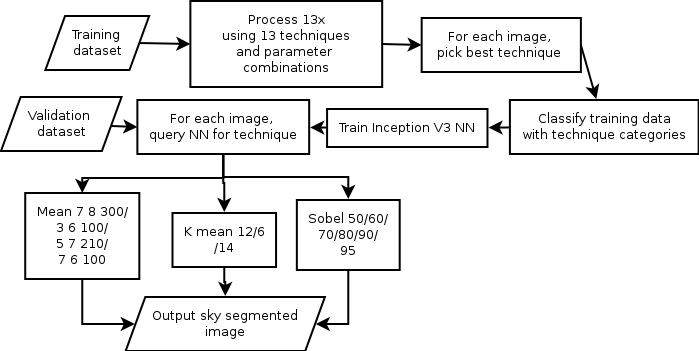
\includegraphics[scale=0.60]{Images/TrainingProcessDiagram}
\caption{\bf Process flow of training and validation steps.}    
 \label{fig:process}  
\end{figure} 

\begin{table}[!htbp]
\caption{\bf Techniques used in this study for sky pixel detection.  \label{tab:techniques}}     
\begin{tabular}{ l l l}
\textbf{Abbreviation} & \textbf{Description} & \textbf{Variations}  \\ \hline
Sobel  & Implementation of \cite{Wang2015a}'s Sobel operator/hybrid probability model & 6 \\	
Mean &  Mean shift segmentation based algorithm developed by the authors &4 \\
K-means  & K-means clustering and HSL colour filtering based algorithm developed by the authors &3 \\
\hline
Sobel/flood-fill  & \cite{Middel2018}'s Sobel operator/flood-fill algorithm used as benchmark &1 \\
\hline
\end{tabular}
\end{table}


\subsection{Data overview}\label{sec:data}
Overall, 38,521 images of outdoor scenes were used. 38,115 images from the Skyfinder dataset were split into two datasets, 28,586 for neural network training and 9529 for validation. An additional 406 images were used from GSV for technique evaluations.

\subsubsection{Skyfinder data}\label{sec:finderdata}
This dataset was built from 90,000 long-term timelapse images from 53 outdoor webcams over a variety of lighting and weather conditions. Images are of a wide range of sizes and aspect ratios, including 640$\times$489, 857$\times$665, 960$\times$600, 1280$\times$720, and 1280$\times$960. For each location, a binary sky mask was created for validation purposes. All of these images are available from the Skyfinder website \citep{Mihail2015}.

In this study, we selected 38,115 images from 40 locations. Night-time and images with heavy fog were removed as these are conditions unlikely to be encountered in imagery used to calculate sky view factor (i.e. Google Street View).

\subsubsection{GSV data}\label{sec:gsvdata}
Panoramas for 406 locations in a variety of cities (Adelaide, Brisbane, Paris, Sydney, Tokyo, Perth, and Melbourne) were retrieved using the Google Maps API \citep{GoogleMaps2017b}. Images were retrieved as six 640$\times$640 tiles (one each for up, down, left, right, front, and back directions). The six images were stitched together into a 1280$\times$960 cubic image using Java 8 \citep{Oracle2018} and OpenCV\citep {Bradski2000}. Validation images were created by hand marking sky regions in each image using the GNU Image Manipulation Program \citep{GIMP2019}. Figure \ref{fig:origmarked} shows an example of an GSV panorama image and a hand-marked validation image.

\begin{figure}
\centering    
\textbf{a)}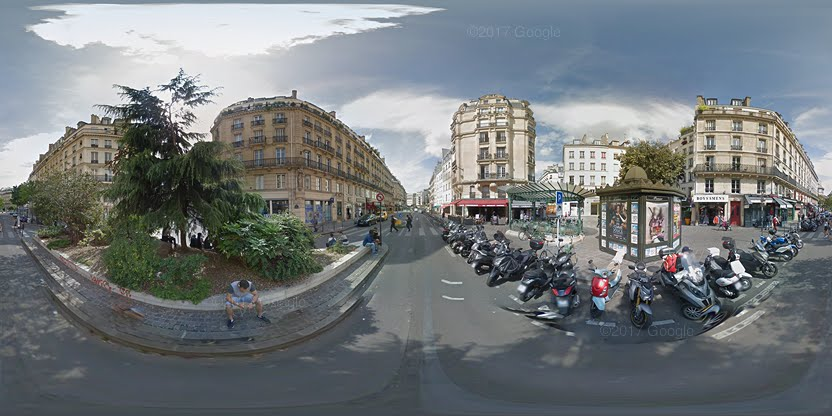
\includegraphics[scale=0.26]{Images/2/panorama-JtVHmEl7WCiz1xJ0bcJpBg-1.png} 
\textbf{b)}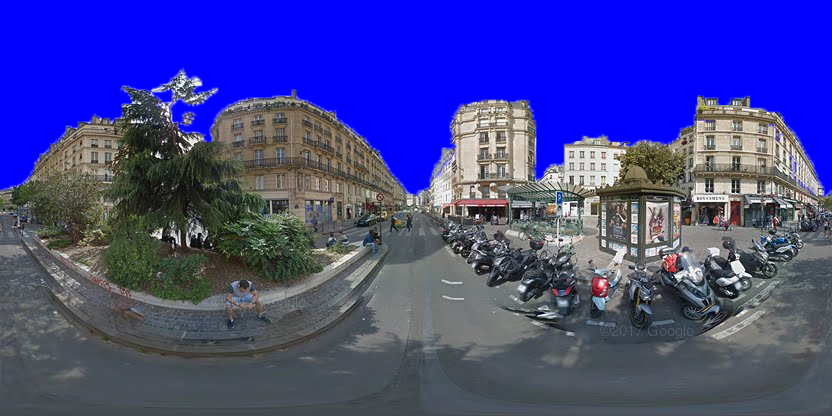
\includegraphics[scale=0.26]{Images/2/panorama-JtVHmEl7WCiz1xJ0bcJpBg-1-marked.png} 

\caption{\bf a) Original panorama image and b) hand-marked validation image.}    
 \label{fig:origmarked}  
\end{figure} 

\subsection{Techniques and parameters}
\subsubsection{\cite{Wang2015a} Sobel operator/hybrid probability model}\label{sec:prob}
An implementation of the sky detection algorithm presented in \cite{Wang2015a} was implemented using OpenCV and Java 8. This method proceeds by calculating grey scale gradient images using x- and y-directional Sobel operators to estimate sky colour. An optimise object function attempts to find the best sky-ground boundary in the gradient image using the covariance matrices of a first calculation of sky and ground regions. Using this best sky boundary, the image is again separated into sky and ground regions and a probability model is created from the centre and standard deviations of the colours. A second probability model is created from the gradient values. A third probability model is built based on the vertical position of each pixel (vertically higher pixels are more likely to be sky). An overall probability model, ranking each pixel's probability (0 to 1) to be sky, is generated from the three probability models. \cite{Wang2015a} reports an error average (in percent of sky) of 0.051 and standard deviation of 0.058 in their evaluation using human-labelled images.  

\cite{Wang2015a} did not recommend a probability threshold, so a number of thresholds were tested (0.5, 0.6, 0.7, 0.8, 0.9, and 0.95) and given the designations of Sobel\_50, Sobel\_60, Sobel\_70, Sobel\_80, Sobel\_90, and Sobel\_95 respectively. The algorithm was applied to each image and pixels that exceeded the chosen threshold were marked as sky pixels (using blue, RGB 0,0,255). Results from our implementation are shown in Figure \ref{fig:sobolresults}. 


%\begin{table}[!htbp]
%\caption{\bf Sobel hybrid probability model designations and parameters used for each  \label{tab:techniques4}}     
%\begin{tabular}{ l l}
%\textbf{Designation}  & \textbf{Threshold}    \\ \hline
%Sobel\_50 & 0.5 \\	  
%Sobel\_60 & 0.6 \\	
%Sobel\_70 & 0.7 \\	
%Sobel\_80 & 0.8 \\
%Sobel\_90 & 0.9 \\
%Sobel\_95 & 0.95 \\
%\hline
%\end{tabular}
%\end{table}



	

\begin{figure}
\centering    
\textbf{a)}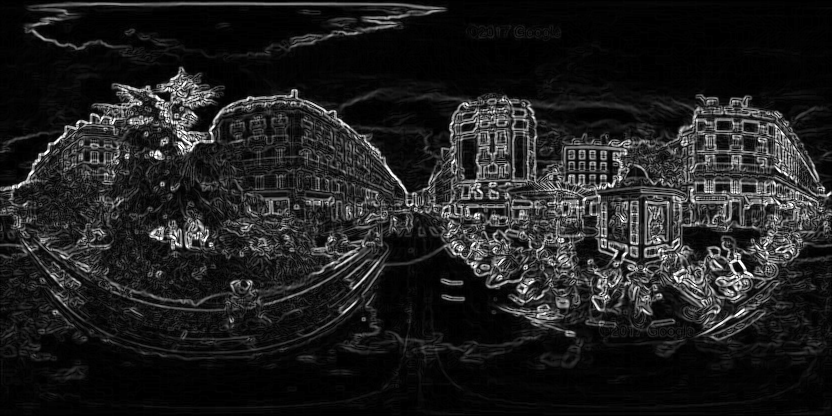
\includegraphics[scale=0.24]{Images/2/panorama-JtVHmEl7WCiz1xJ0bcJpBg-1_Sobel.png} 
\textbf{b)}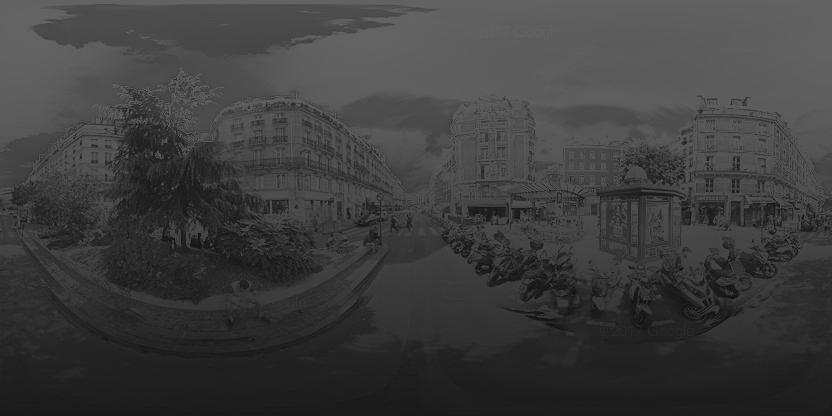
\includegraphics[scale=0.24]{Images/2/panorama-JtVHmEl7WCiz1xJ0bcJpBg-1_Sobel_prob.png} 
\textbf{c)}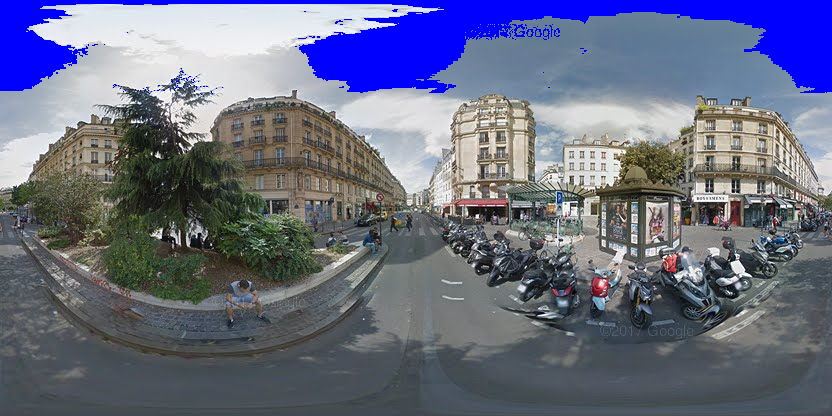
\includegraphics[scale=0.24]{Images/2/panorama-JtVHmEl7WCiz1xJ0bcJpBg-1_Sobel_95_marked.png} 
\textbf{d)}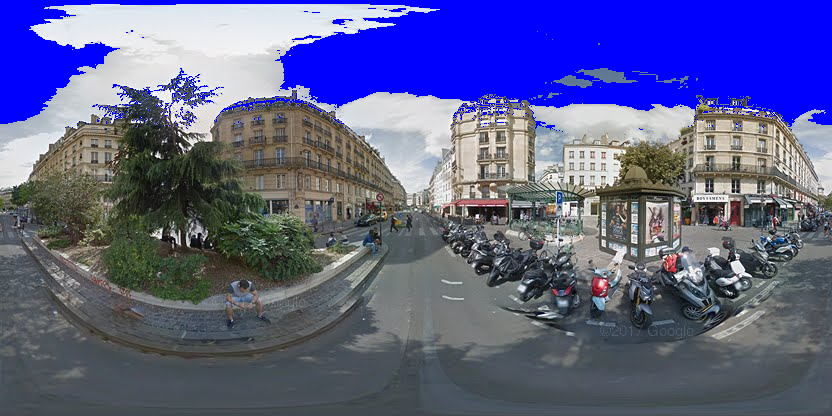
\includegraphics[scale=0.24]{Images/2/panorama-JtVHmEl7WCiz1xJ0bcJpBg-1_Sobel_90_marked.png} 
\textbf{e)}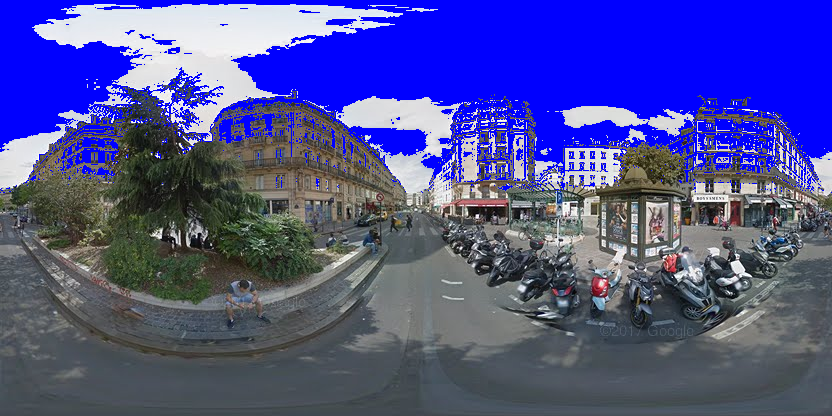
\includegraphics[scale=0.24]{Images/2/panorama-JtVHmEl7WCiz1xJ0bcJpBg-1_Sobel_80_marked.png} 
\textbf{f)}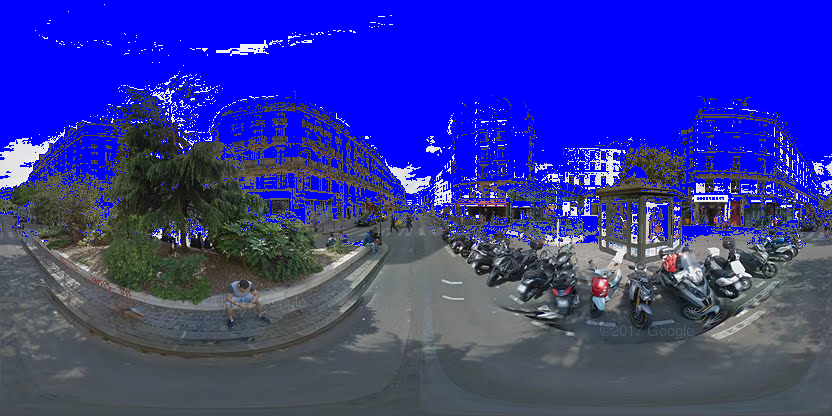
\includegraphics[scale=0.24]{Images/2/panorama-JtVHmEl7WCiz1xJ0bcJpBg-1_Sobel_70_marked.png} 
\textbf{g)}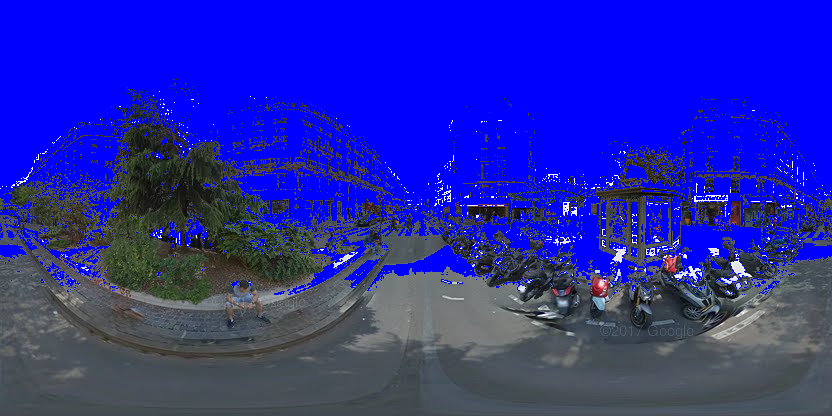
\includegraphics[scale=0.24]{Images/2/panorama-JtVHmEl7WCiz1xJ0bcJpBg-1_Sobel_60_marked.png} 
\textbf{h)}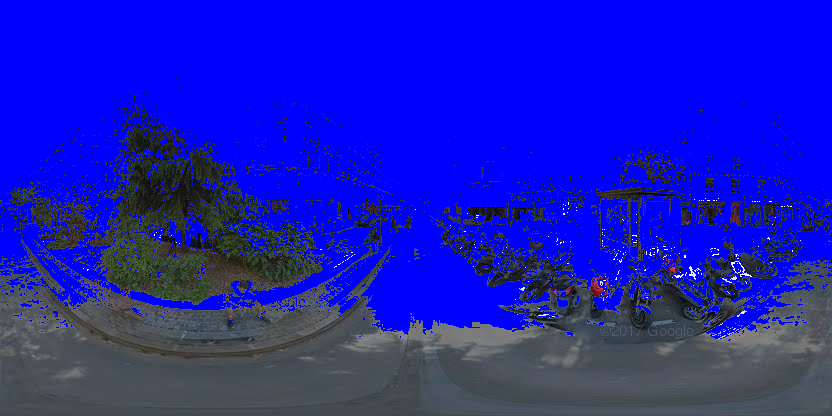
\includegraphics[scale=0.24]{Images/2/panorama-JtVHmEl7WCiz1xJ0bcJpBg-1_Sobel_50_marked.png} 
\caption{\bf  Results of Sobel operator/hybrid probability model, showing a) Sobel operator gradient image, b) resulting probability predictions, c) Sobel\_50, d) Sobel\_60, e) Sobel\_70, f) Sobel\_80, g) Sobel\_90, and h) Sobel\_95.}    
 \label{fig:sobolresults}  
\end{figure} 

\subsubsection{Mean shift segmentation algorithm}\label{sec:mean}

Mean shift is an algorithm often used for image segmentation \citep{Comaniciu1997,Comaniciu2002}. Image segmentation involves decomposing images into homogeneous contiguous regions of pixels of similar colours or grey levels. Mean shift uses an iterative algorithm to pick search windows (spatial and range) of a certain radius in an initial location in an image, then compute a mean shift vector and translate the search window by that amount until convergence \citep{Comaniciu1997}. Segmentation results are highly dependent on input parameters for the algorithm, which include the spatial radius of the search window, colour range radius of the search window, and minimum density (the minimum number of pixels to constitute a region). The mean shift used in this project is based on a Java port by \cite{Pangburn2002} of the C++ based EDISON vision toolkit \citep{Christoudias2002}. 

Four different variations of the input parameters were used, determined experimentally through a sensitivity test to work across the widest variety of images. For example, in an effort to shift the entire sky to a single colour, images with patchy multi-coloured clouds are more accurately segmented when the radius and density parameters are increased (in Figures \ref{fig:meantypes}a to \ref{fig:meantypes}d). However, this can have the effect of creating false positives in other images, for example, buildings (in Figures \ref{fig:meantypes}i to \ref{fig:meantypes}l, centre left background) are increasingly segmented into the sky. The technique designations and parameters are detailed in Table \ref{tab:techniques2}. Mean shift is applied to each image with the chosen set of parameters and pixels of the most common colour (in the top half of the segmented image) are marked as sky. Results are shown in Figure \ref{fig:meanresults}.


\begin{table}[!htbp]
\caption{\bf Mean shift segmentation algorithm designations and parameters (units in pixels) used for each \label{tab:techniques2}}     
\begin{tabular}{ l l l l}
\textbf{Designation}  & \textbf{Spatial radius}&\textbf{Range radius}&\textbf{Min. density}   \\ \hline
Mean\_7\_8\_300 & 7& 8& 300 \\
Mean\_3\_6\_100	& 3& 6& 100 \\
Mean\_5\_7\_210	& 5& 7& 210 \\	 
Mean\_7\_6\_100	& 7& 6& 100 \\

\hline
\end{tabular}
\end{table}



\begin{figure}
\centering    
\textbf{\phantom{\textbf{a)}}}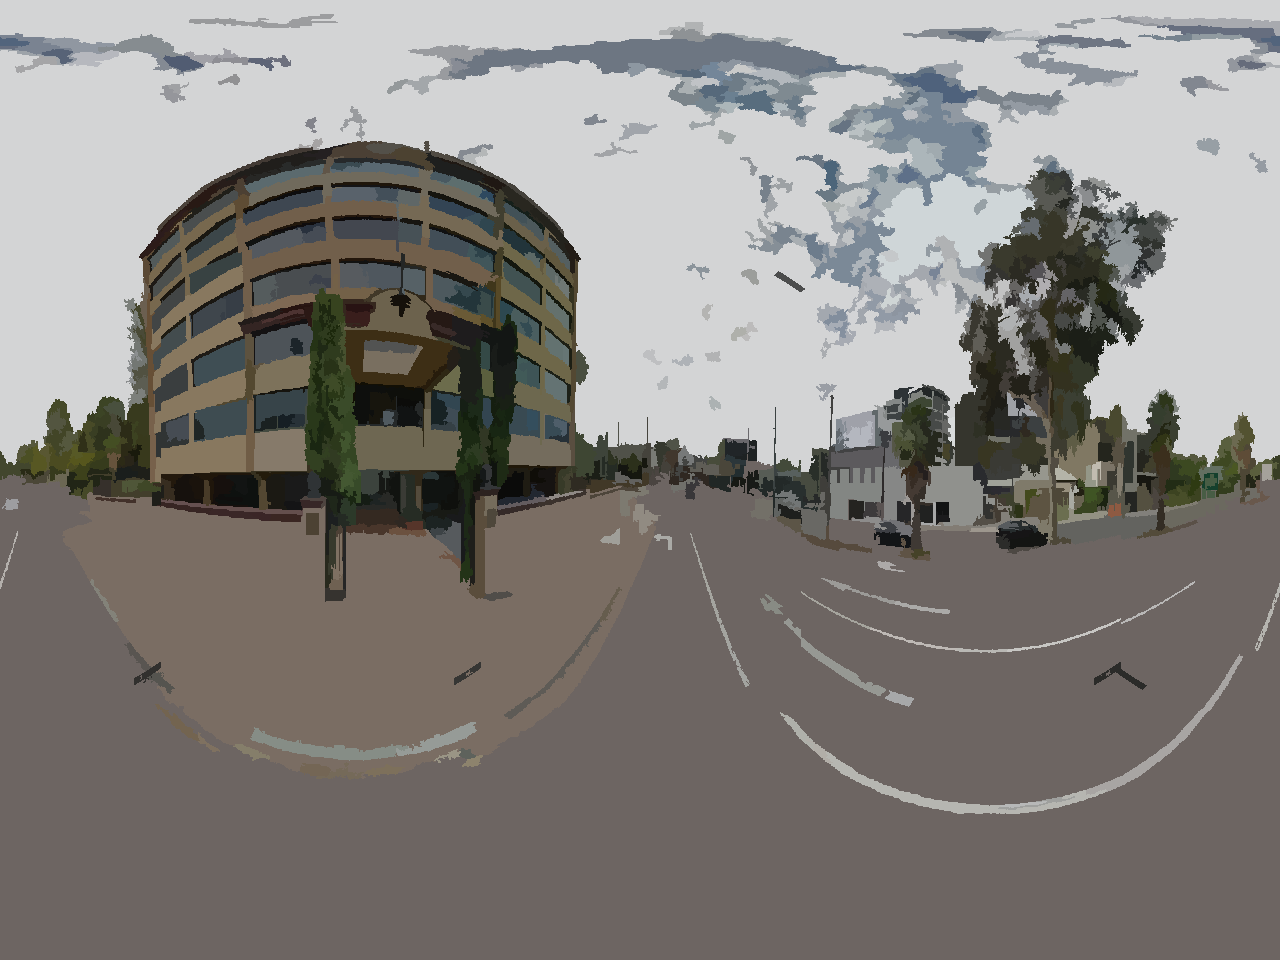
\includegraphics[scale=0.08]{Images/mean/4880_3_6_100.png} 
\textbf{\phantom{\textbf{b)}}}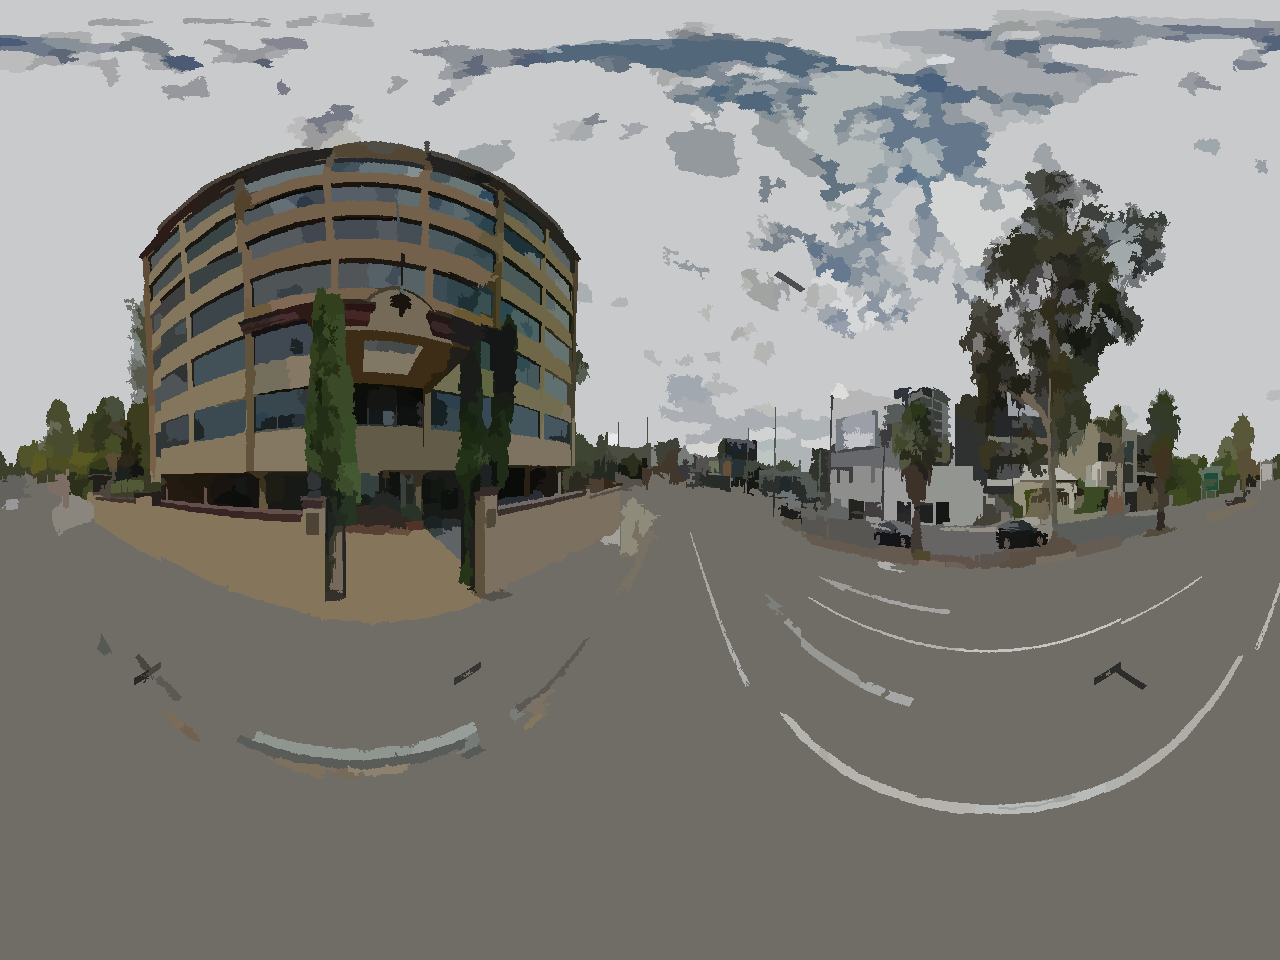
\includegraphics[scale=0.08]{Images/mean/4880_7_6_100.png} 
\textbf{\phantom{\textbf{c)}}}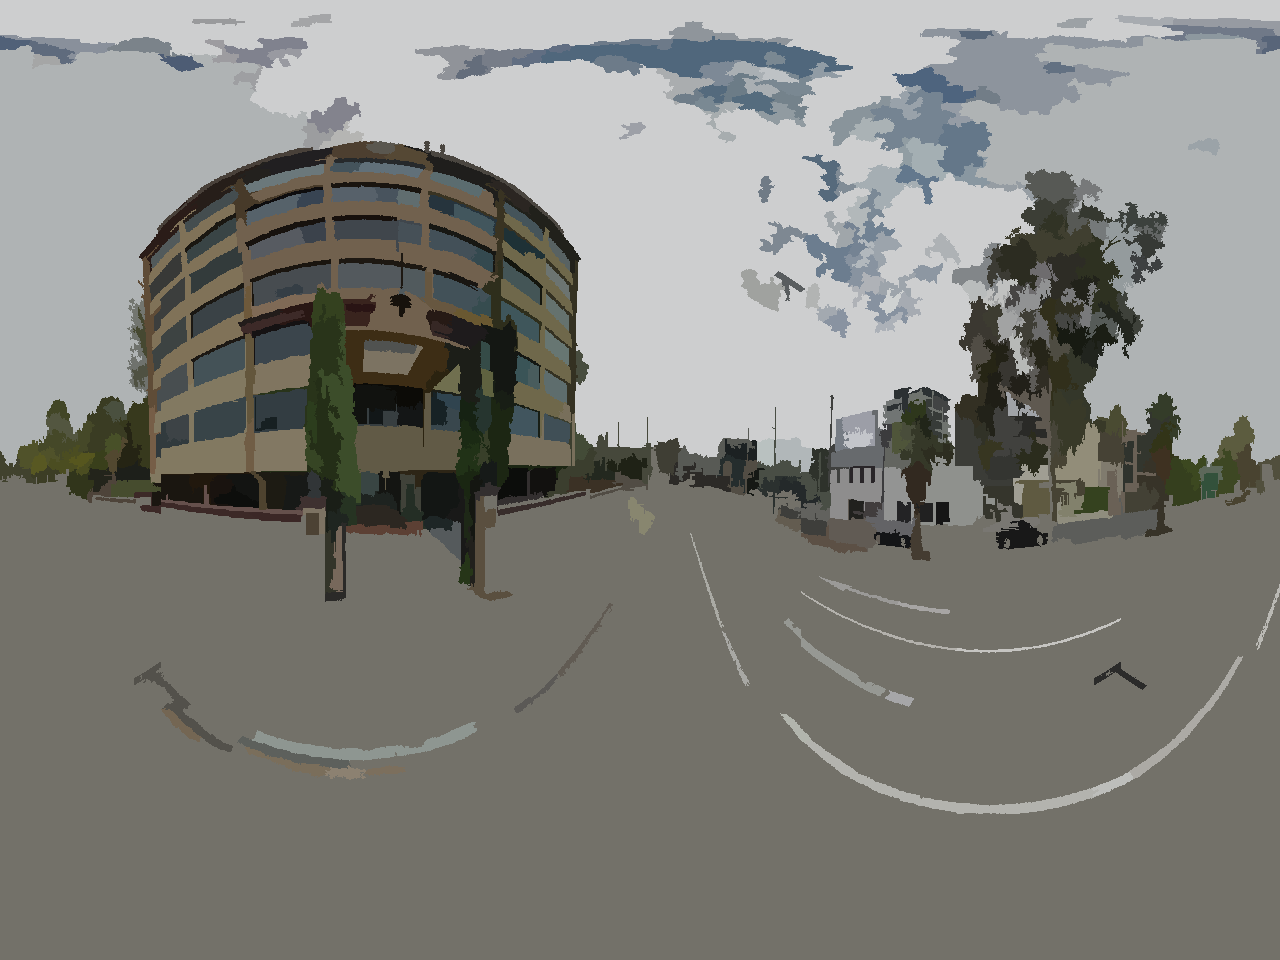
\includegraphics[scale=0.08]{Images/mean/4880_5_7_210.png} 
\textbf{\phantom{\textbf{d)}}}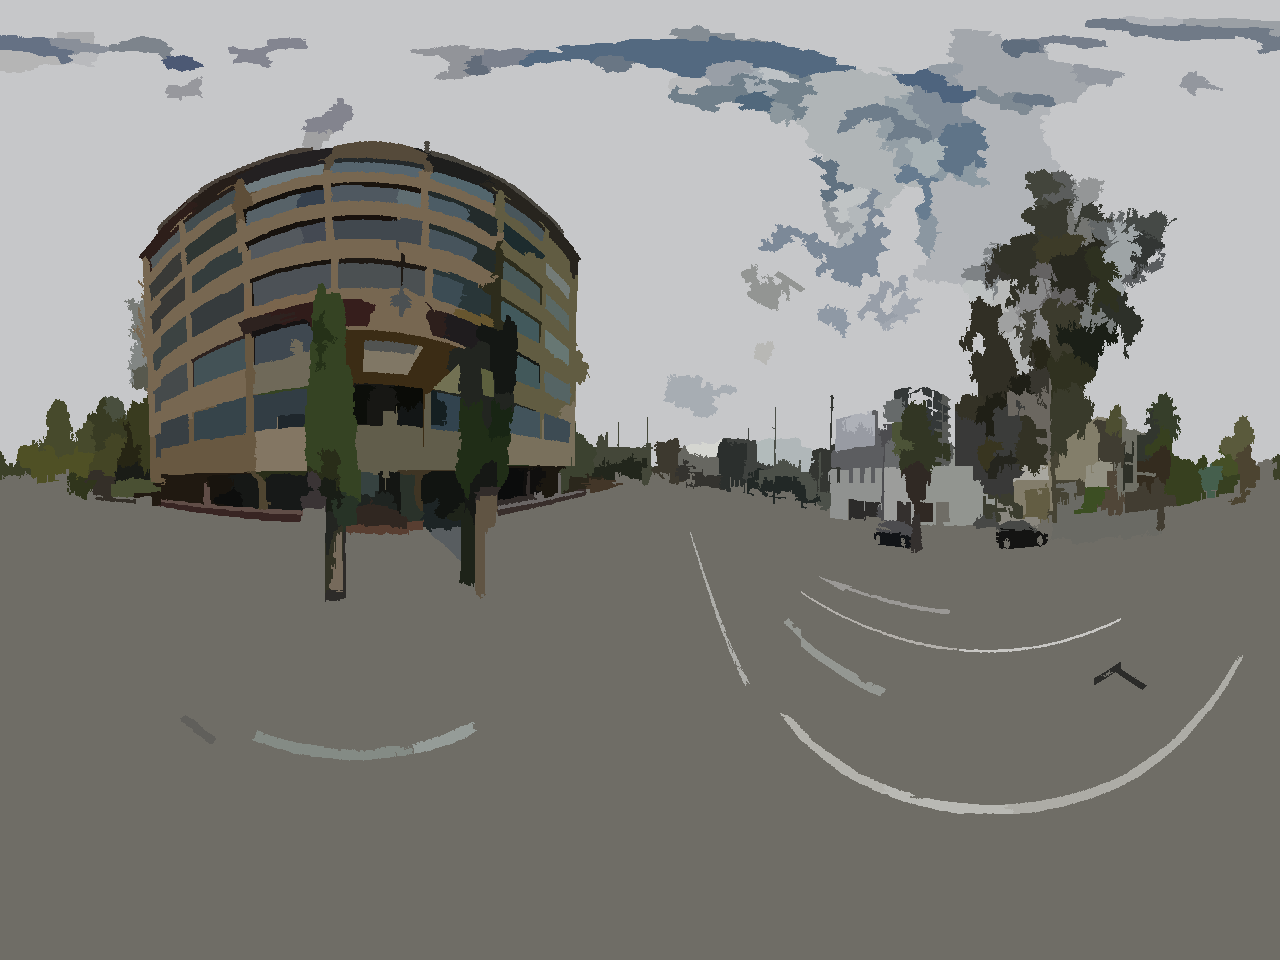
\includegraphics[scale=0.08]{Images/mean/4880_7_8_300.png} 1)
\textbf{\phantom{\textbf{a)}}}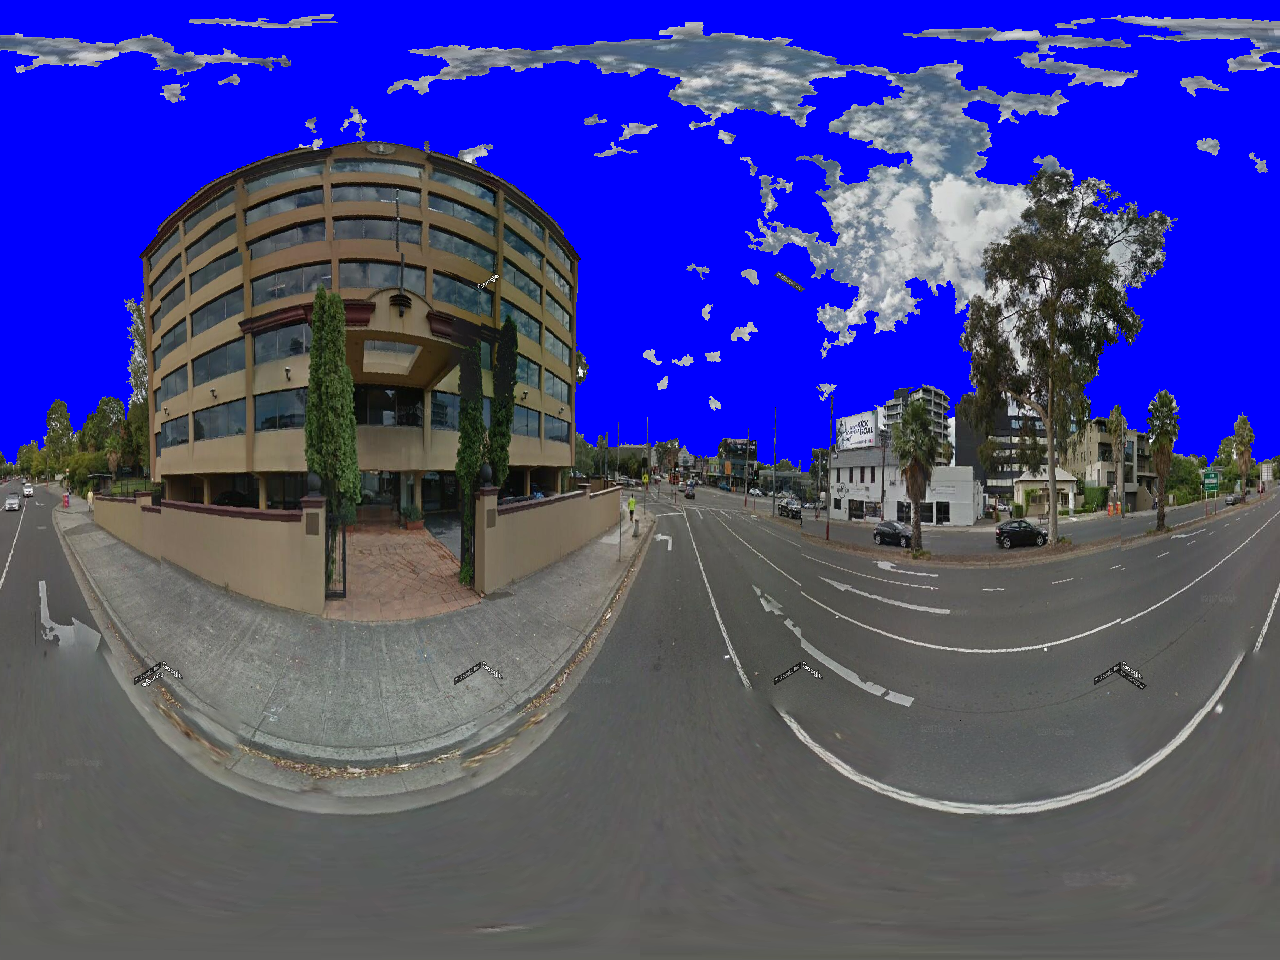
\includegraphics[scale=0.08]{Images/mean/4880_3_6_100_ms_sky_mark.png} 
\textbf{\phantom{\textbf{b)}}}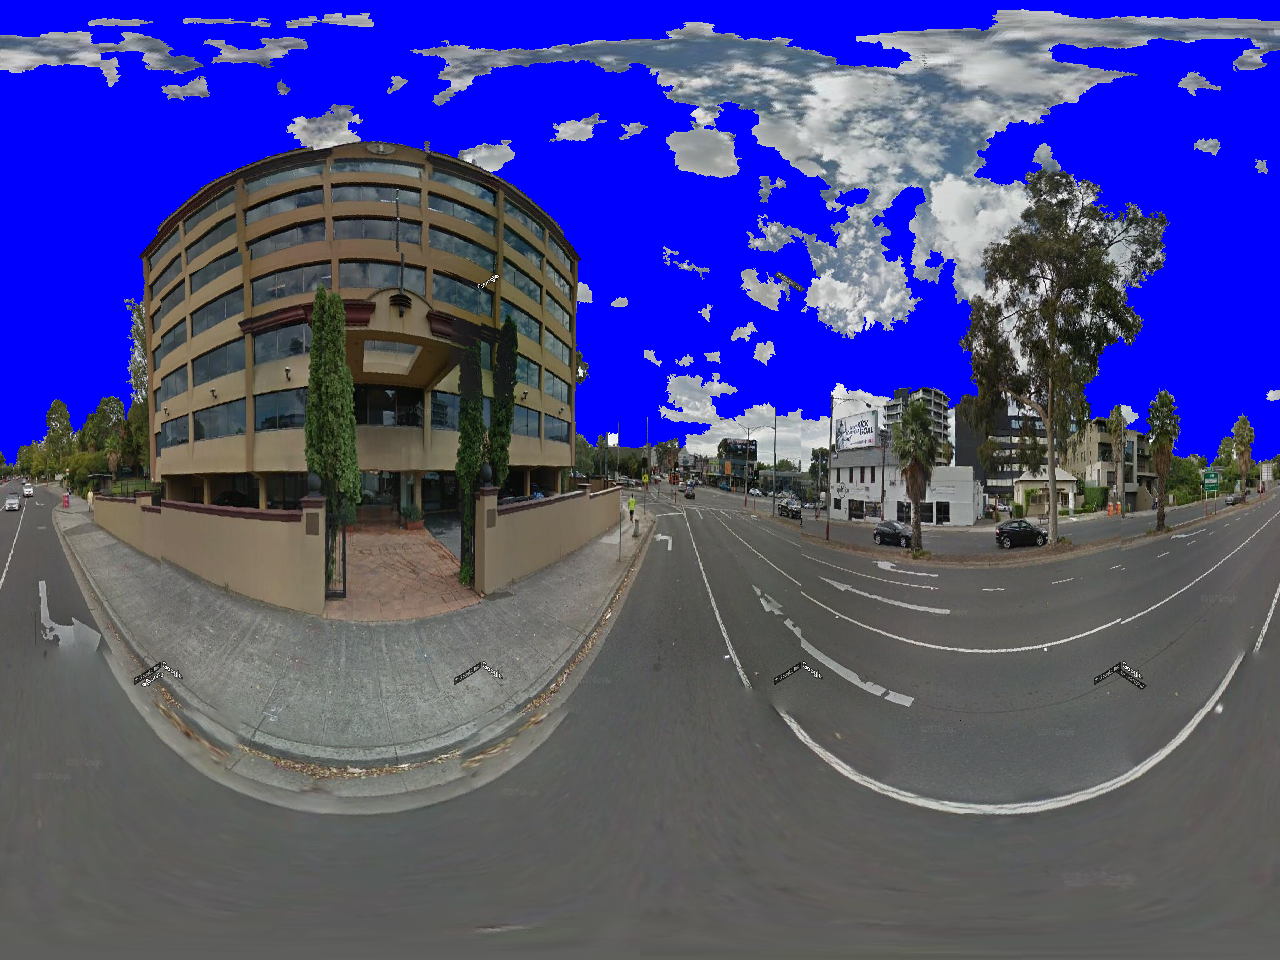
\includegraphics[scale=0.08]{Images/mean/4880_7_6_100_ms_sky_mark.png} 
\textbf{\phantom{\textbf{c)}}}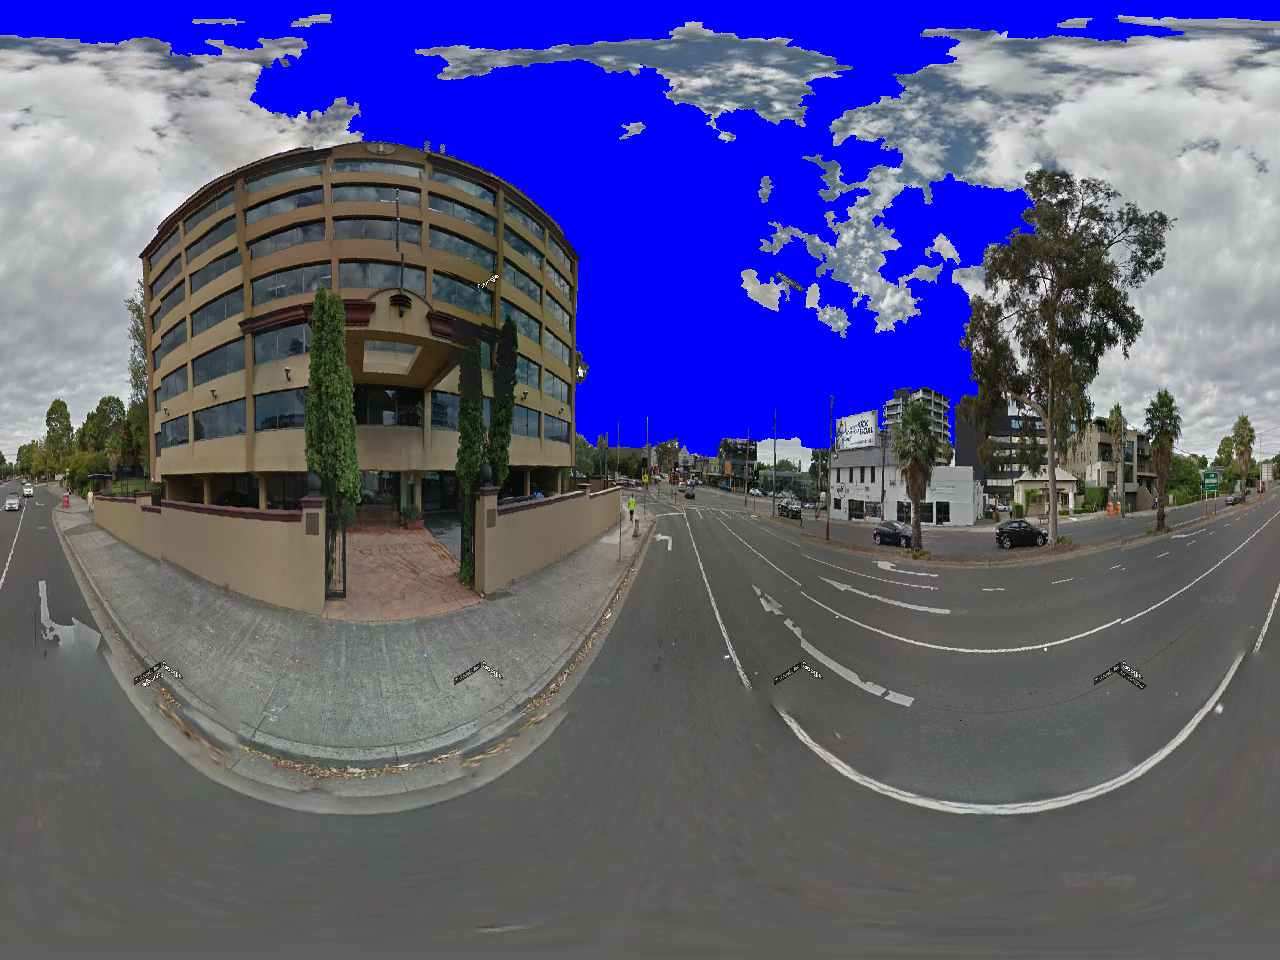
\includegraphics[scale=0.08]{Images/mean/4880_5_7_210_ms_sky_mark.png} 
\textbf{\phantom{\textbf{d)}}}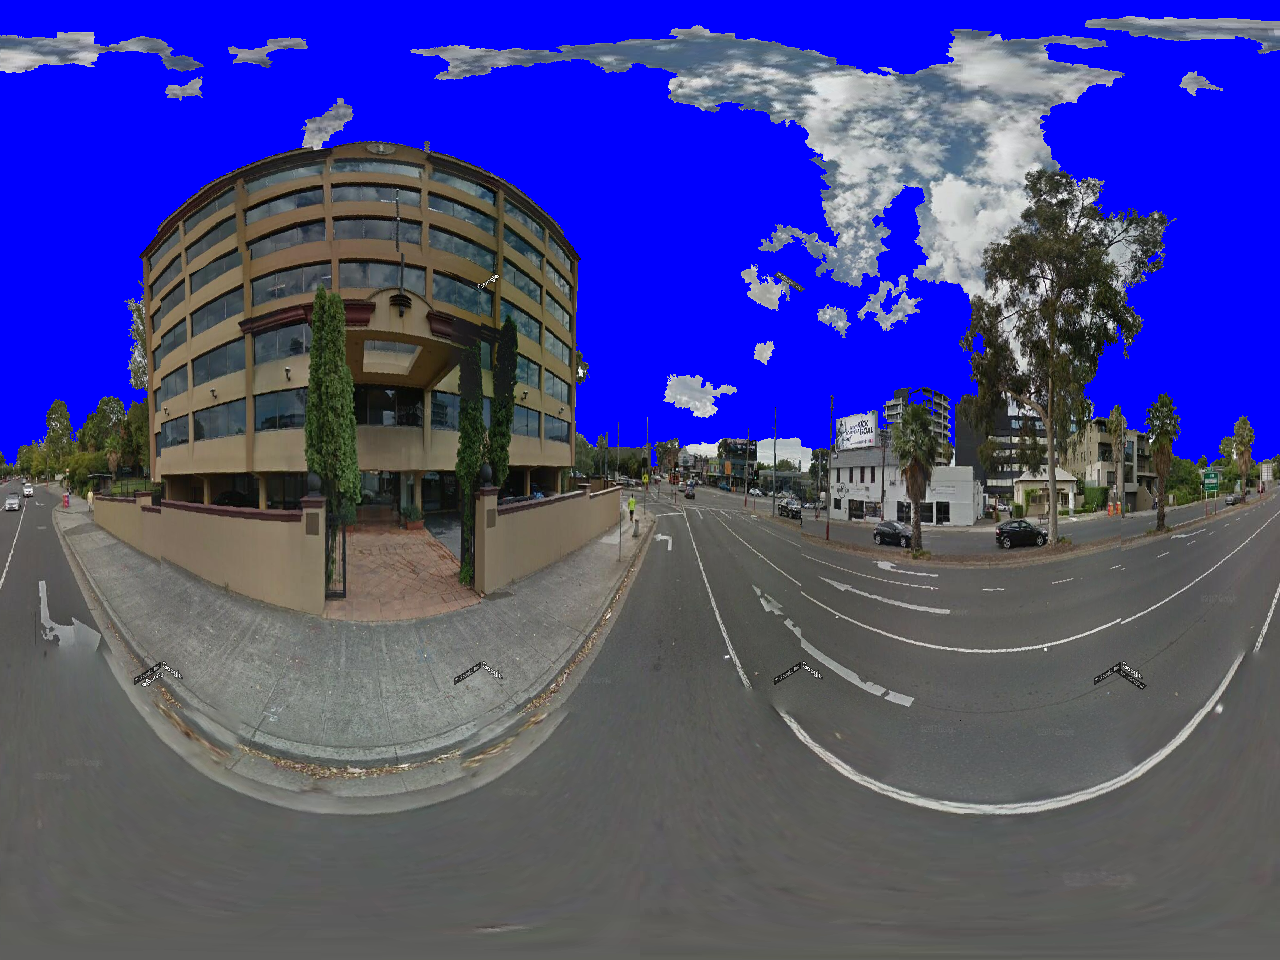
\includegraphics[scale=0.08]{Images/mean/4880_7_8_300_ms_sky_mark.png} 2)
\textbf{\phantom{\textbf{a)}}}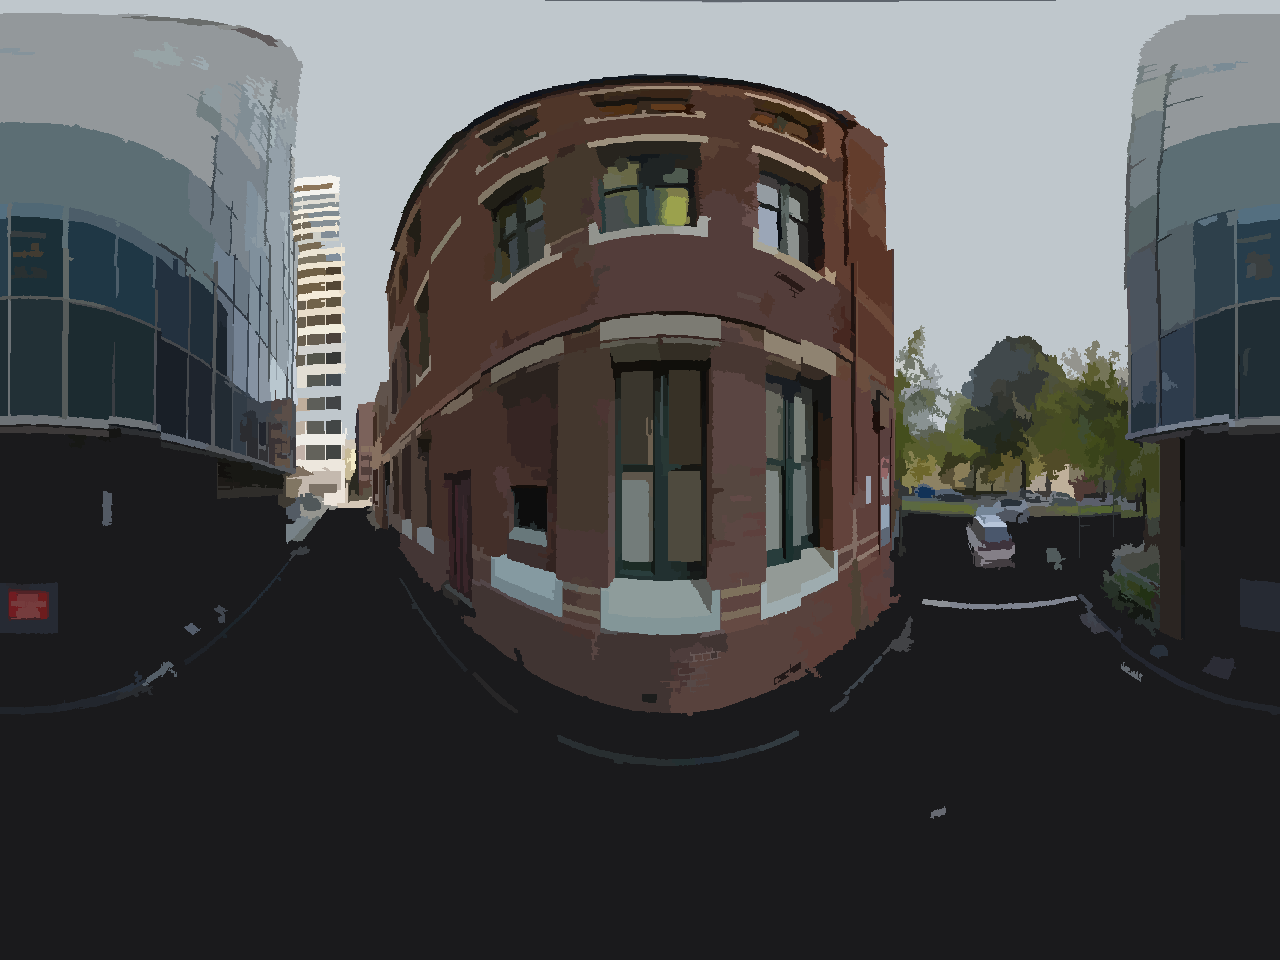
\includegraphics[scale=0.08]{Images/mean/0070_3_6_100.png} 
\textbf{\phantom{\textbf{b)}}}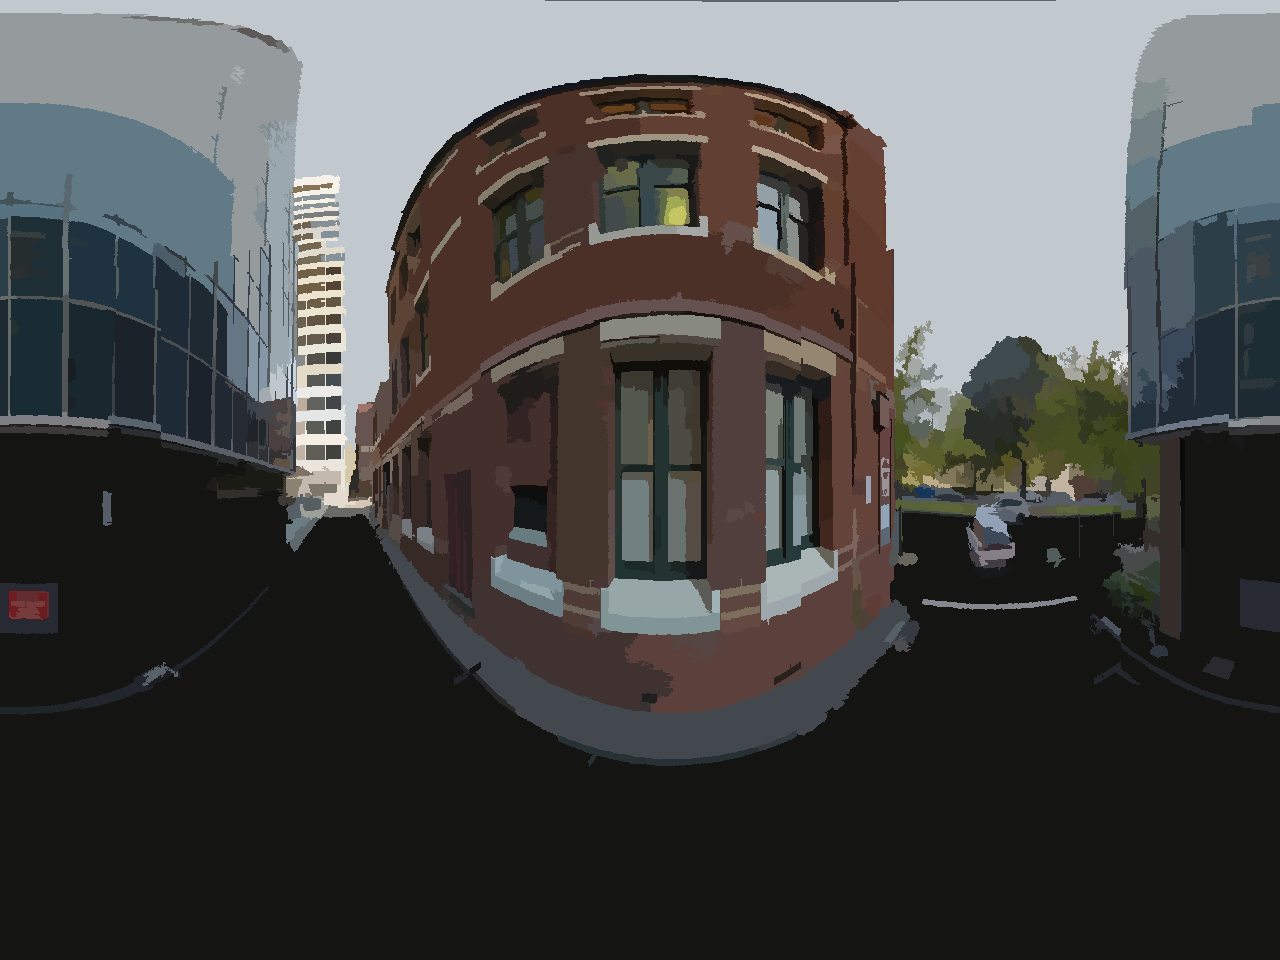
\includegraphics[scale=0.08]{Images/mean/0070_7_6_100.png} 
\textbf{\phantom{\textbf{c)}}}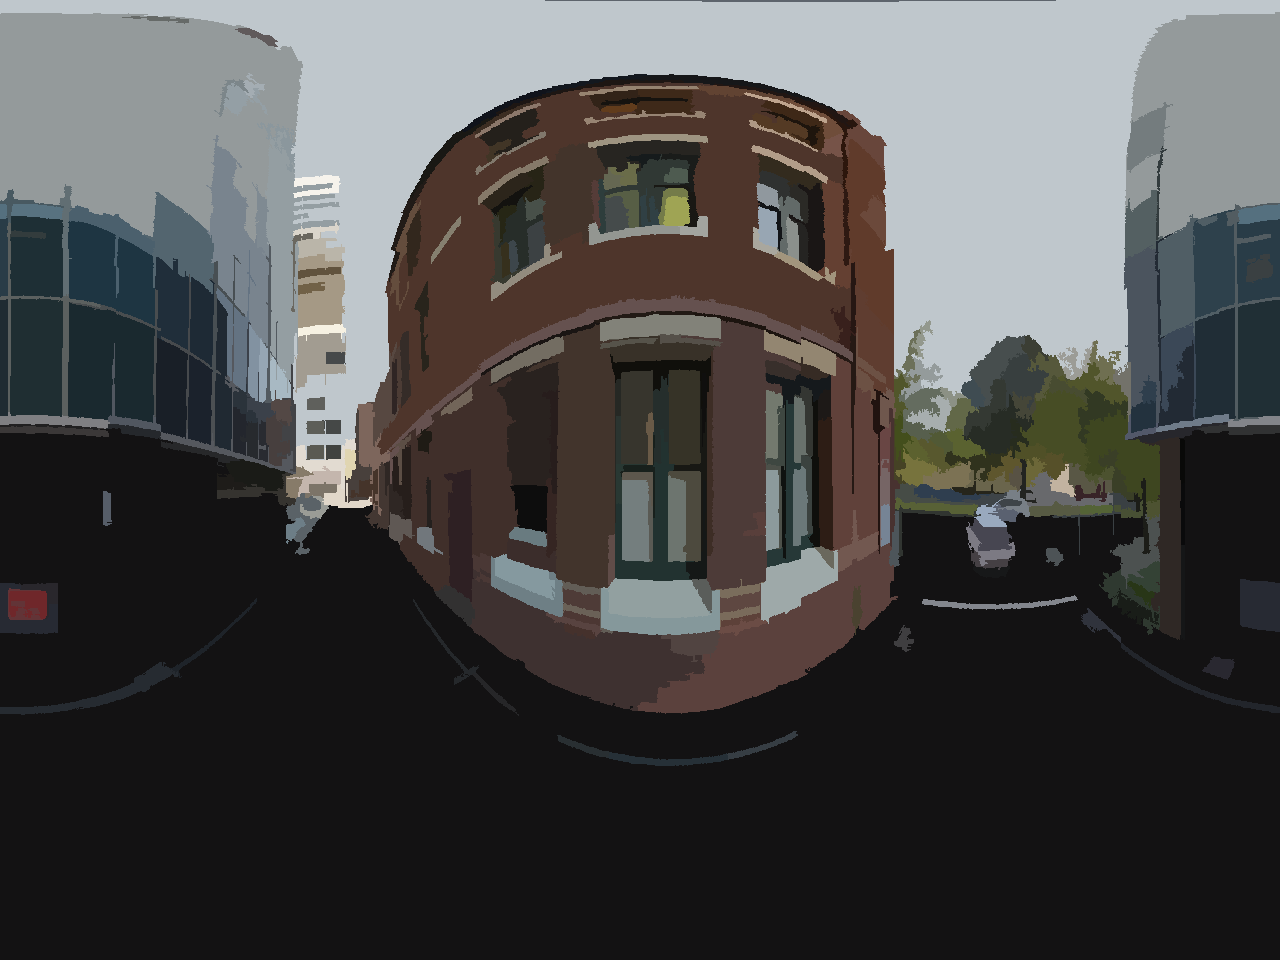
\includegraphics[scale=0.08]{Images/mean/0070_5_7_210.png} 
\textbf{\phantom{\textbf{d)}}}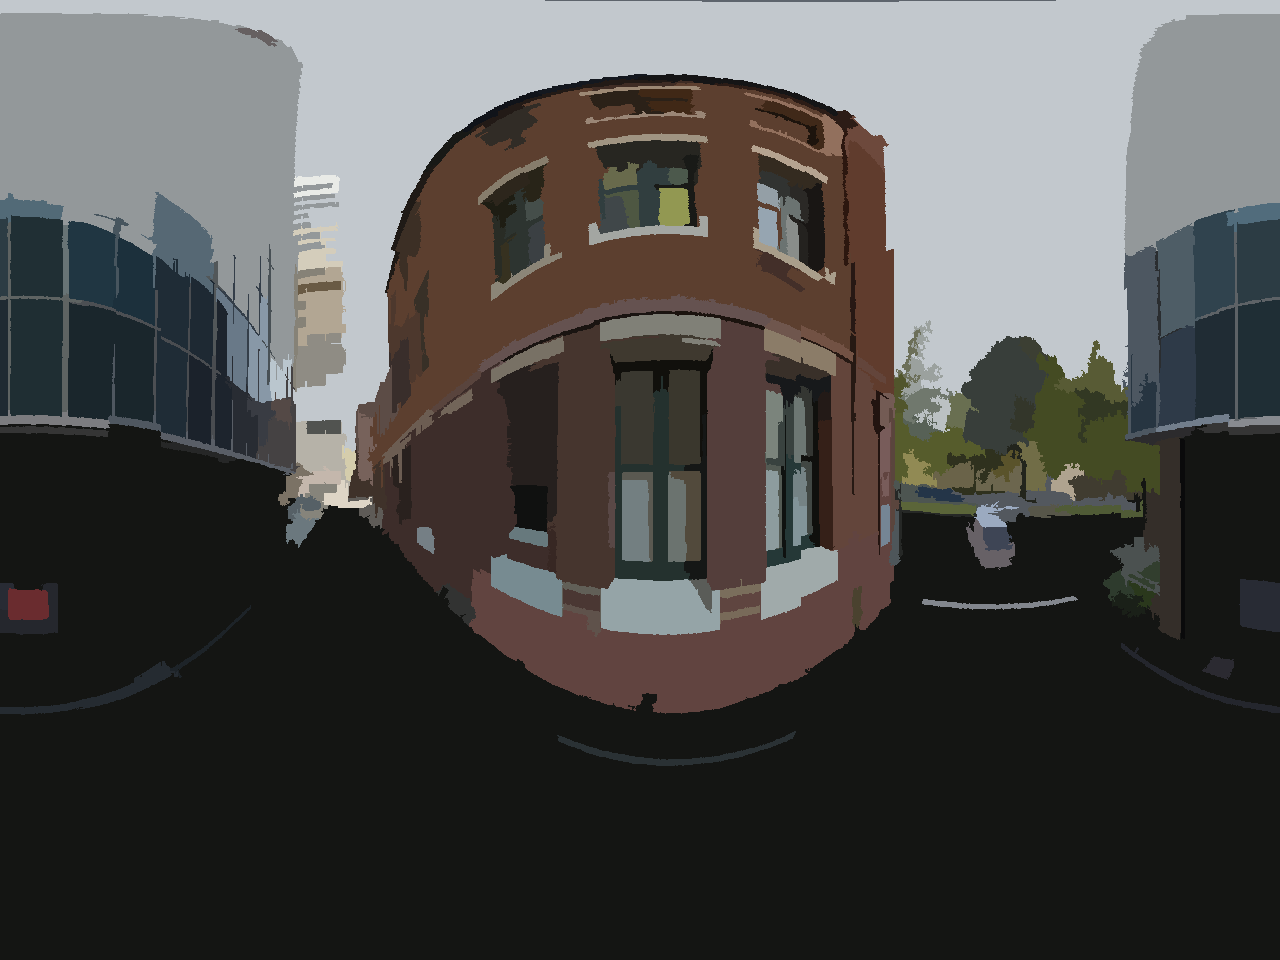
\includegraphics[scale=0.08]{Images/mean/0070_7_8_300.png} 3)
\textbf{a)}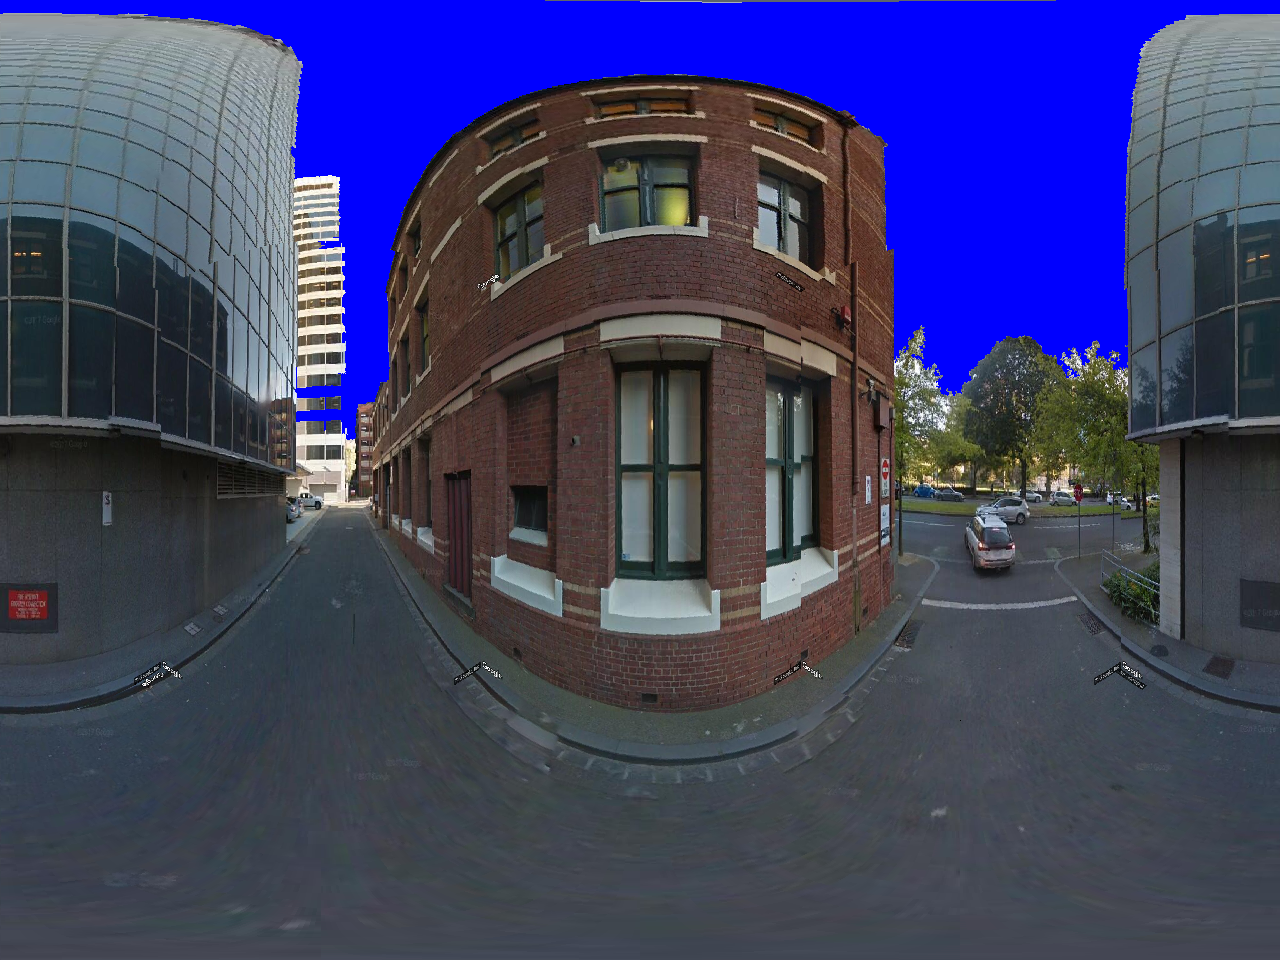
\includegraphics[scale=0.08]{Images/mean/0070_3_6_100_ms_sky_mark.png} 
\textbf{b)}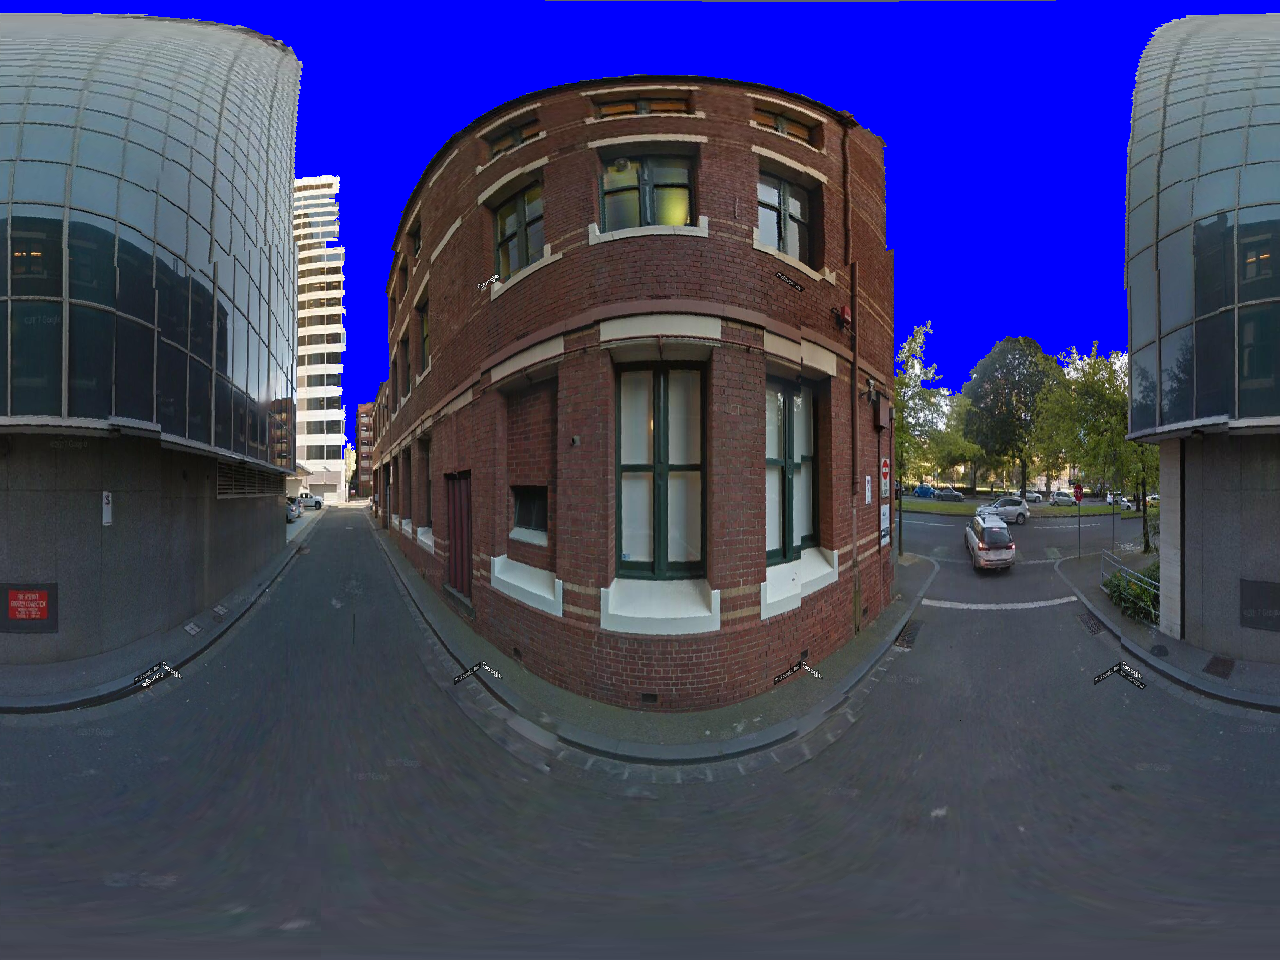
\includegraphics[scale=0.08]{Images/mean/0070_7_6_100_ms_sky_mark.png} 
\textbf{c)}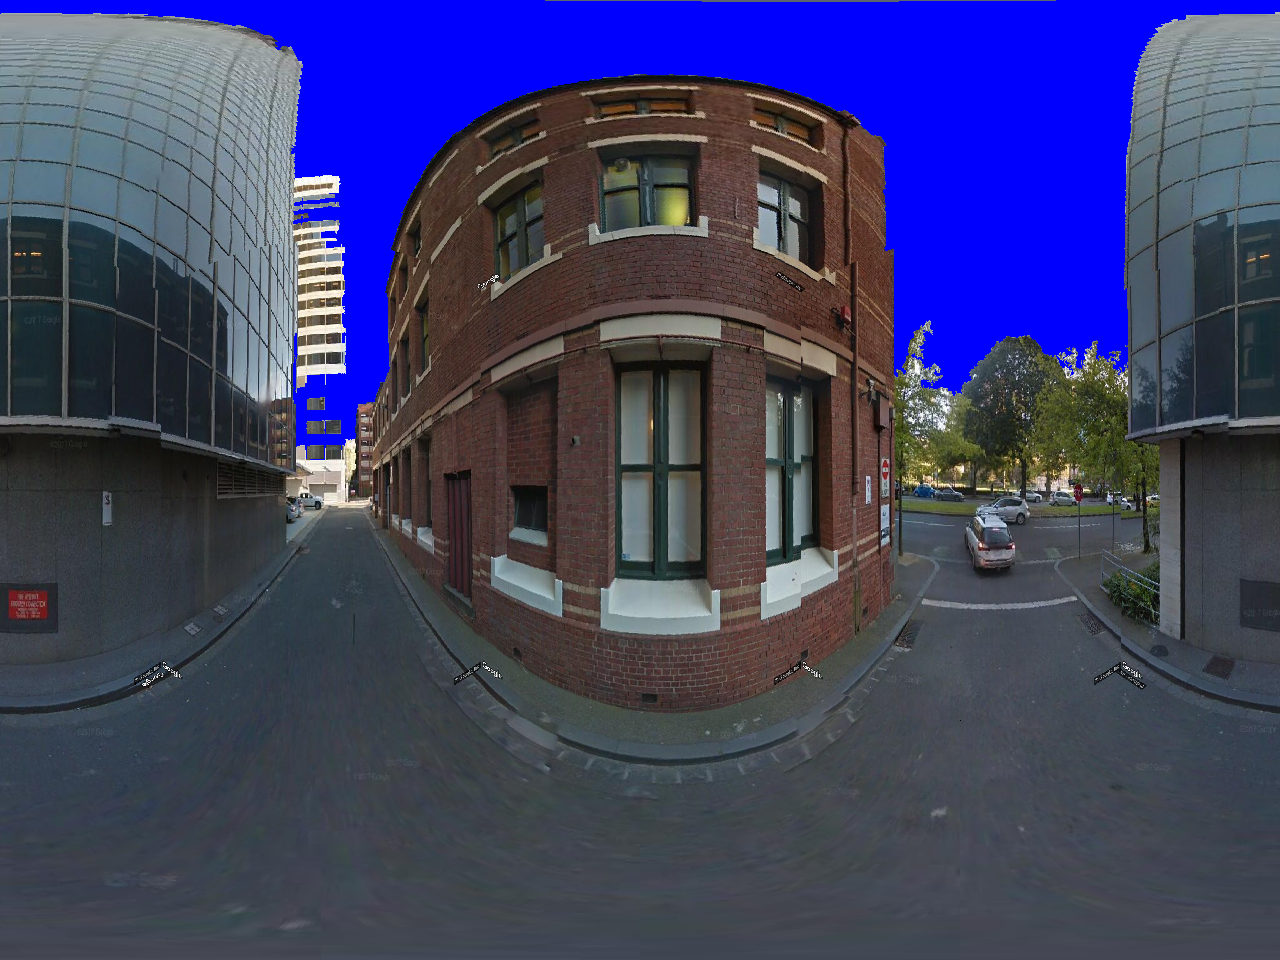
\includegraphics[scale=0.08]{Images/mean/0070_5_7_210_ms_sky_mark.png} 
\textbf{d)}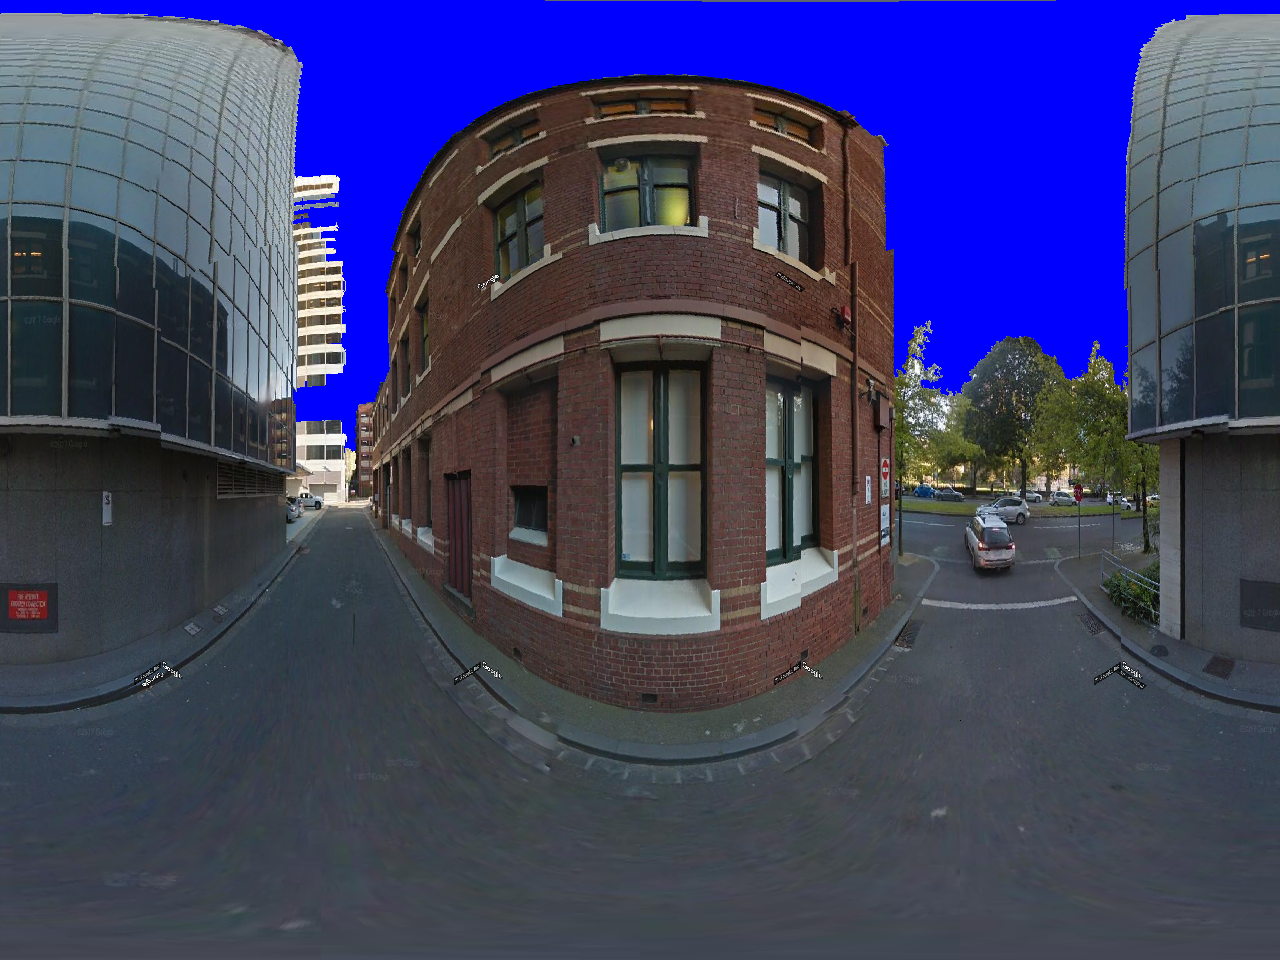
\includegraphics[scale=0.08]{Images/mean/0070_7_8_300_ms_sky_mark.png} 4)

\caption{\bf Comparison outputs of intermediate mean shift segmentation algorithm processing steps using varying parameters, showing columns a) Mean\_3\_6\_100, b) Mean\_7\_6\_100, c) Mean\_5\_7\_210, d) Mean\_7\_8\_300 and rows 1) and 3) intermediate mean shifted and rows 2) and 4) the final marked images. }
 \label{fig:meantypes}  
\end{figure} 




\begin{figure}
\centering    
\textbf{a)}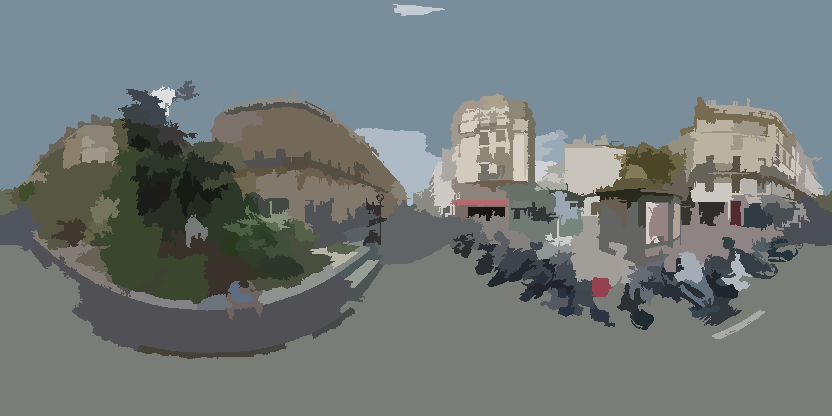
\includegraphics[scale=0.26]{Images/2/panorama-JtVHmEl7WCiz1xJ0bcJpBg-1_seg.png} 
\textbf{b)}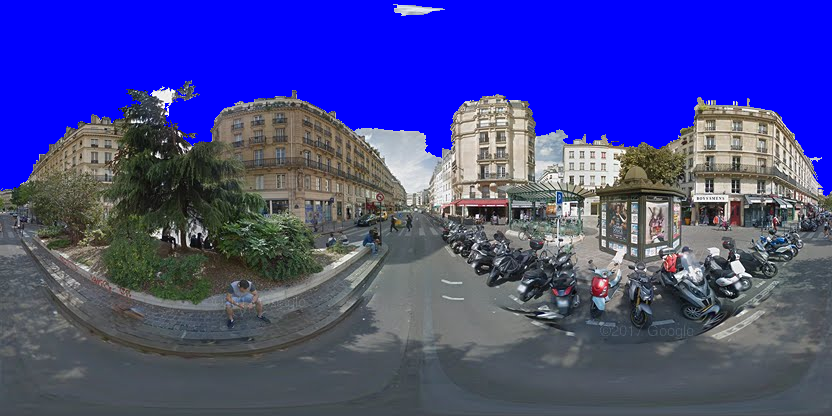
\includegraphics[scale=0.26]{Images/2/panorama-JtVHmEl7WCiz1xJ0bcJpBg-1_ms_sky_mark.png} 
\caption{\bf Results of mean shift segmentation algorithm (Mean\_5\_7\_210) showing a) mean shifted image and b) final marked image.}    
 \label{fig:meanresults}  
\end{figure} 



\subsubsection{K-means clustering and HSL color filtering}\label{sec:kmeans}
A third sky segmentation technique was designed using K-means clustering and hue, saturation, and lightness (HSL) colour filtering. K-means clustering iteratively splits an image into $K$ number of clusters, terminating when a specified criteria is met (i.e. maximum iterations and/or desired accuracy). The K-means clustering was performed using the K-means method from the OpenCV library. Three different input parameter settings were used, determined experimentally through a sensitivity test to work on a wide variety of images. The technique designations and parameters are detailed in Table \ref{tab:techniques3}. K-mean\_12 was found to work best when the sky is mostly obscured by a building or bridge. K-mean\_6 is more accurate with cloudy skies. K-mean\_14 handles a sky scene broken up by tree canopies.

K-means clustering was performed on each image, splitting the image into the chosen number of clusters. Filtering cluster regions was based on HSL values. The following conditions (for $H$, hue, $S$, saturation, and $L$, lightness) must be met to add a colour region to a list of possible sky regions: 

$H_{low} < H < H_{high}$

$\cup L > L_{lightness}$

$\cup L > L_{grey} \cap S < S_{grey}$

Of these possible sky clusters, only clusters with a number of pixels greater than the $Skyreq$ threshold (percent of all pixels) in the image were finally marked as sky regions. Example results are shown in Figure \ref{fig:kmeansresults}. 

\begin{table}[!htbp]
\caption{\bf K-means clustering and HSL color filtering designations and parameters used for each \label{tab:techniques3}}     
\begin{tabular}{ l l l l l l l l}
\textbf{Designation} & \textbf{Clusters} & \textbf{Skyreq}&\textbf{H$_{high}$}&\textbf{H$_{low}$} & \textbf{L$_{lightness}$} & \textbf{L$_{grey}$}& \textbf{S$_{grey}$} \\ \hline
K-mean\_12  & 12 & 0.7& 0.75& 0.3 & 0.95 & 0.75 & 0.2 \\
K-mean\_6  & 6 & 0.6& 0.75& 0.3 & 0.95 & 0.75 & 0.2 \\
K-mean\_14  & 14 & 0.4& 0.75& 0.3 & 0.95 & 0.65 & 0.2 \\
\hline
\end{tabular}
\end{table}

\begin{figure}
\centering    
%\textbf{a)}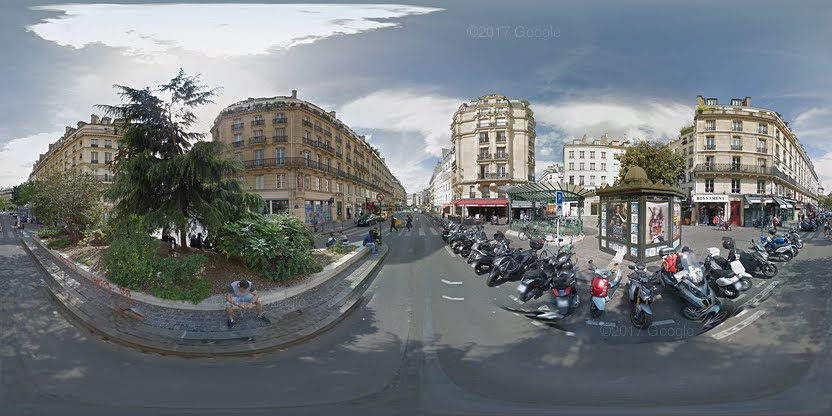
\includegraphics[scale=0.20]{Images/2/Cloudy/panorama-JtVHmEl7WCiz1xJ0bcJpBg-1_cropped.png} 
\textbf{a)}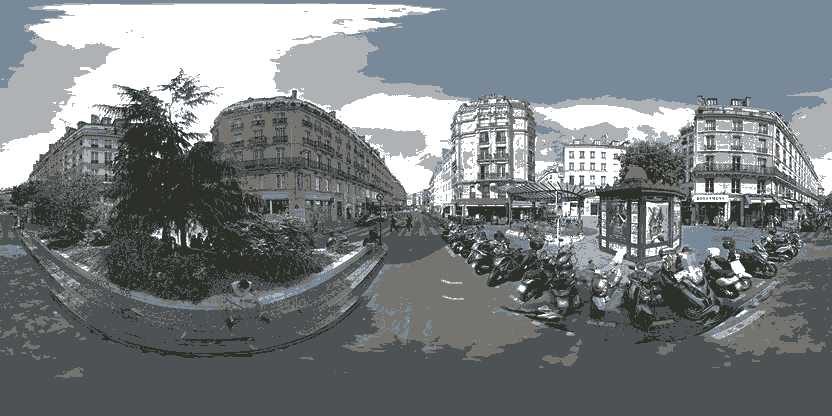
\includegraphics[scale=0.17]{Images/2/Cloudy/panorama-JtVHmEl7WCiz1xJ0bcJpBg-1_clustered6.png} 
\textbf{b)}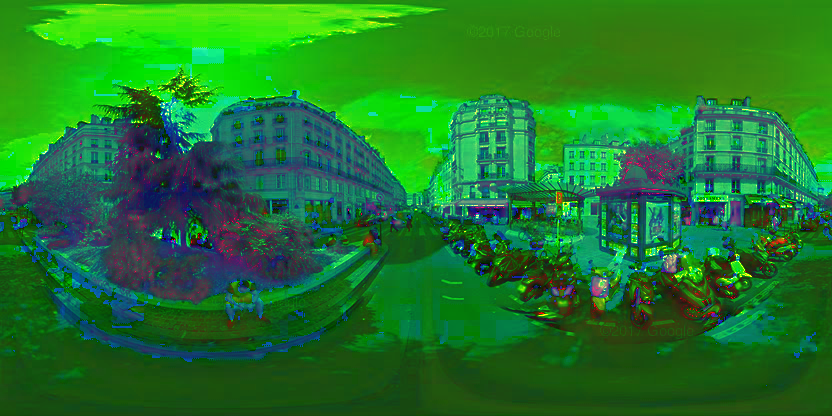
\includegraphics[scale=0.17]{Images/2/Cloudy/panorama-JtVHmEl7WCiz1xJ0bcJpBg-1_HLS6.png} 
\textbf{c)}\includegraphics[scale=0.17]{Images/2/Cloudy/{panorama-JtVHmEl7WCiz1xJ0bcJpBg-1_sky_mark0.4}.png} 
\caption{\bf  Results of K-means clustering and HSL color filtering (K-mean\_6), showing a) K-means clustered image, b) HSL intermediate image, and c) final marked image.}    
 \label{fig:kmeansresults}  
\end{figure} 



\subsubsection{\cite{Middel2018} Sobel operator/flood-fill algorithm}\label{sec:floodfill}

\cite{Middel2018} developed a process based on a Sobel filter \citep{Sobel1968} and flood-fill algorithm \citep{Laungrungthip2008,Middel2017}. This method was designed to calculate sky view factor from Google Street View panoramas that had the bottom half cropped off and converted to a fisheye projection. Note, this algorithm also rescales the imagery to 512$\times$512. All 38,521 images in the combined training and validation dataset were processed with this algorithm (sky pixels marked with white, RGB 255,255,255), compared to validation images, and results saved for a comparison with our process flow results. These results were kept separate from the other 13 techniques and were not included in the NN training process (see Section \ref{sec:nntraining}). Also, in this benchmark comparison, we used this system to process a varied outdoor imagery dataset, not the fisheye imagery (cropped below the horizon) this algorithm was originally designed to process. Results are shown in Figure \ref{fig:sobelflood}.



\begin{figure}
\centering    
\textbf{a)}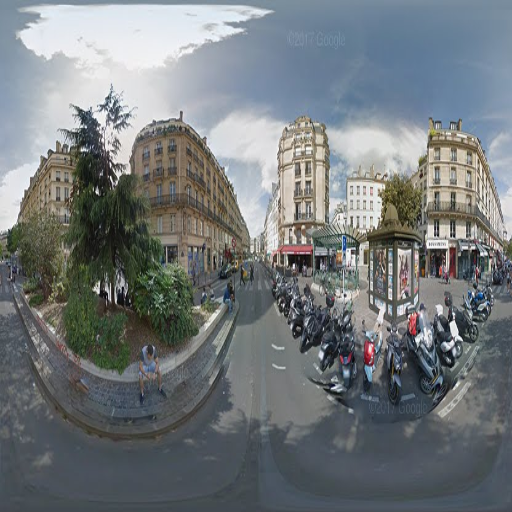
\includegraphics[scale=0.27]{Images/2/FloodfillInput.png}
\textbf{b)}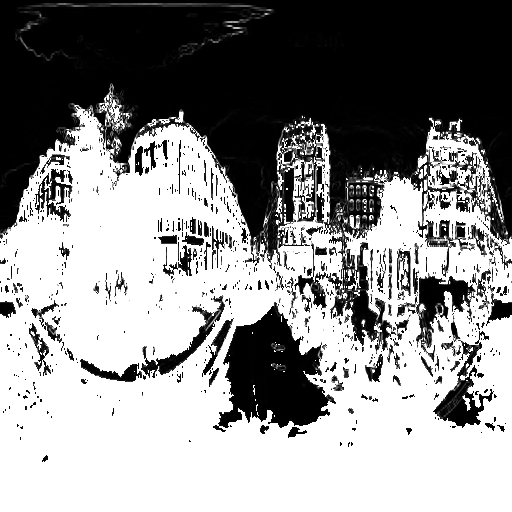
\includegraphics[scale=0.27]{Images/2/FloodfillMiddle.png}
\textbf{c)}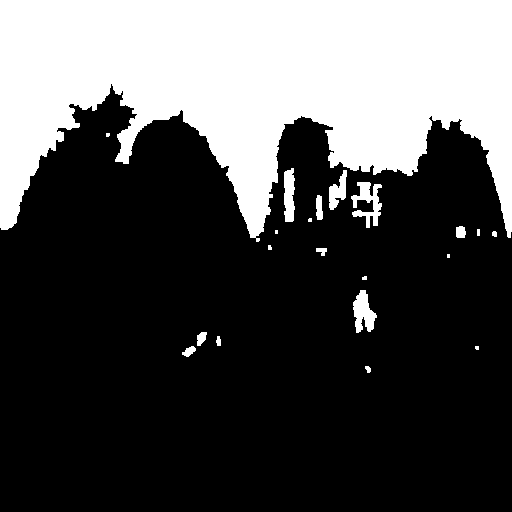
\includegraphics[scale=0.27]{Images/2/FloodfillOutput.png}
\caption{\bf   Results of Sobel/flood-fill combination, showing a) original image (rescaled to 512x512), b) intermediate Sobel image, and c) final marked sky image.}    
 \label{fig:sobelflood}  
\end{figure} 

\subsection{Neural network}\label{sec:nn}

\subsubsection{Inception V3}\label{sec:inception}
The Microsoft Cognitive Toolkit (CNTK) \citep{Yu2015,Agarwal2016}, with the the Inception V3 network \citep{Szegedy2015a}, was used in this project to route images through our adaptive algorithm. This artificial neural network (NN) is a widely used model for image classification across a large variety of fields \citep{Xia2017,Hassannejad2016}. The model was trained by presenting it with a list of images assigned to categories (in our case which technique performed most accurately for each image) and running the training process until the model reached peak accuracy (convergence) at recognising images from these classifications.


\subsubsection{Neural network training}\label{sec:nntraining}    

The Skyfinder dataset of 38,115 images was split into two datasets of 75\% training and 25\% validation. All training and validation images (which consisted of images of a wide variety of sizes and aspect ratios) were rescaled to 300$\times$300. The network was calibrated using supervised learning with the generated dataset to identify one of the 13 sky detection techniques variations that performed with the highest accuracy for each image. Note, none of the GSV imagery was used in the NN training process.





\subsubsection{Neural network inference}\label{sec:nninference}    
Using the trained model, inferences were performed using the images from the validation dataset (the 25\% of images from Section \ref{sec:nntraining}) as well as the 406 GSV panoramas. Based on the classification picked by the NN as being the most probable, the appropriate technique and parameters from that classification were used to mark the sky pixels. The marked sky pixels were compared to the ground truth to assess accuracy.



\section{Results}\label{sec:results}

%Overall, 38,521 images were used, 38,115 from the Skyfinder dataset and 406 from Google Street View. During the training and evaluation, the two datasets were combined then split into 28,886 training and 9635 validation images.

There are three sets of results reported in this section. The first is a comparison of all of the techniques and parameters run individually against the Skyfinder and GSV datasets (a total of 38,521 images). The second presents the results of 9636  validation images using our process flow with the techniques and parameters chosen by the trained NN. The third presents a comparison to two benchmark models: a) the \cite{Wang2015a} Sobel operator/hybrid probability model and b) the \cite{Middel2018} Sobel operator/flood-fill algorithm.

\subsection{Results from all techniques}\label{sec:resultsall}
All the technique and parameter variations were used to process the two datasets of the 38,115 Skyfinder, 406 GSV images. A summary of R$^{2}$ and RMSE statistics for evaluations against the two datasets is presented in Table \ref{tab:evalall}. Plots of a number of the better performing techniques are presented in Figure \ref{fig:errorallcombined}. Note, the strong horizontal lines in these figures are due to the nature of the dataset that contain large groups of the same scenes (with the same percentage of sky) under different lighting and weather conditions, resulting in a wide range of calculated results.

\begin{table}[!htbp]
\caption{\bf Evaluation of all techniques and parameters for Skyfinder dataset and GSV dataset. \label{tab:evalall}}     
\begin{tabular}{ l  l l l l }
\textbf{Designation}  & \textbf{Skyfinder R$^{2}$} & \textbf{Skyfinder RMSE} & \textbf{GSV R$^{2}$} & \textbf{GSV RMSE}  \\ \hline
Mean\_3\_6\_100	&0.658&0.148&0.603&0.062 \\
Mean\_5\_7\_210	&0.659&0.142&0.526&0.069 \\
Mean\_7\_6\_100	&0.748&0.104&0.525&0.072 \\
Mean\_7\_8\_300 &0.646&0.143&0.544&0.067  \\
K-mean\_6       &0.023&0.325&0.002&0.16 \\
K-mean\_12      &0.028&0.343&0.017&0.264 \\
K-mean\_14      &0.029&0.328&0.023&0.233 \\
Sobel\_50       &0.104&0.23 &0.026&0.302 \\
Sobel\_60       &0.288&0.164&0.005&0.189 \\
Sobel\_70       &0.396&0.134&0.049&0.108 \\
Sobel\_80       &0.255&0.177&0.433&0.07  \\
Sobel\_90       &0.041&0.317&0.214&0.142 \\
Sobel\_95       &0    &0.421&0.053&0.224 \\
\hline
Sobel/flood-fill&0.134&0.211&0.067&0.312 \\
\hline
\end{tabular}
\end{table}



\begin{figure}
\centering
\textbf{a)}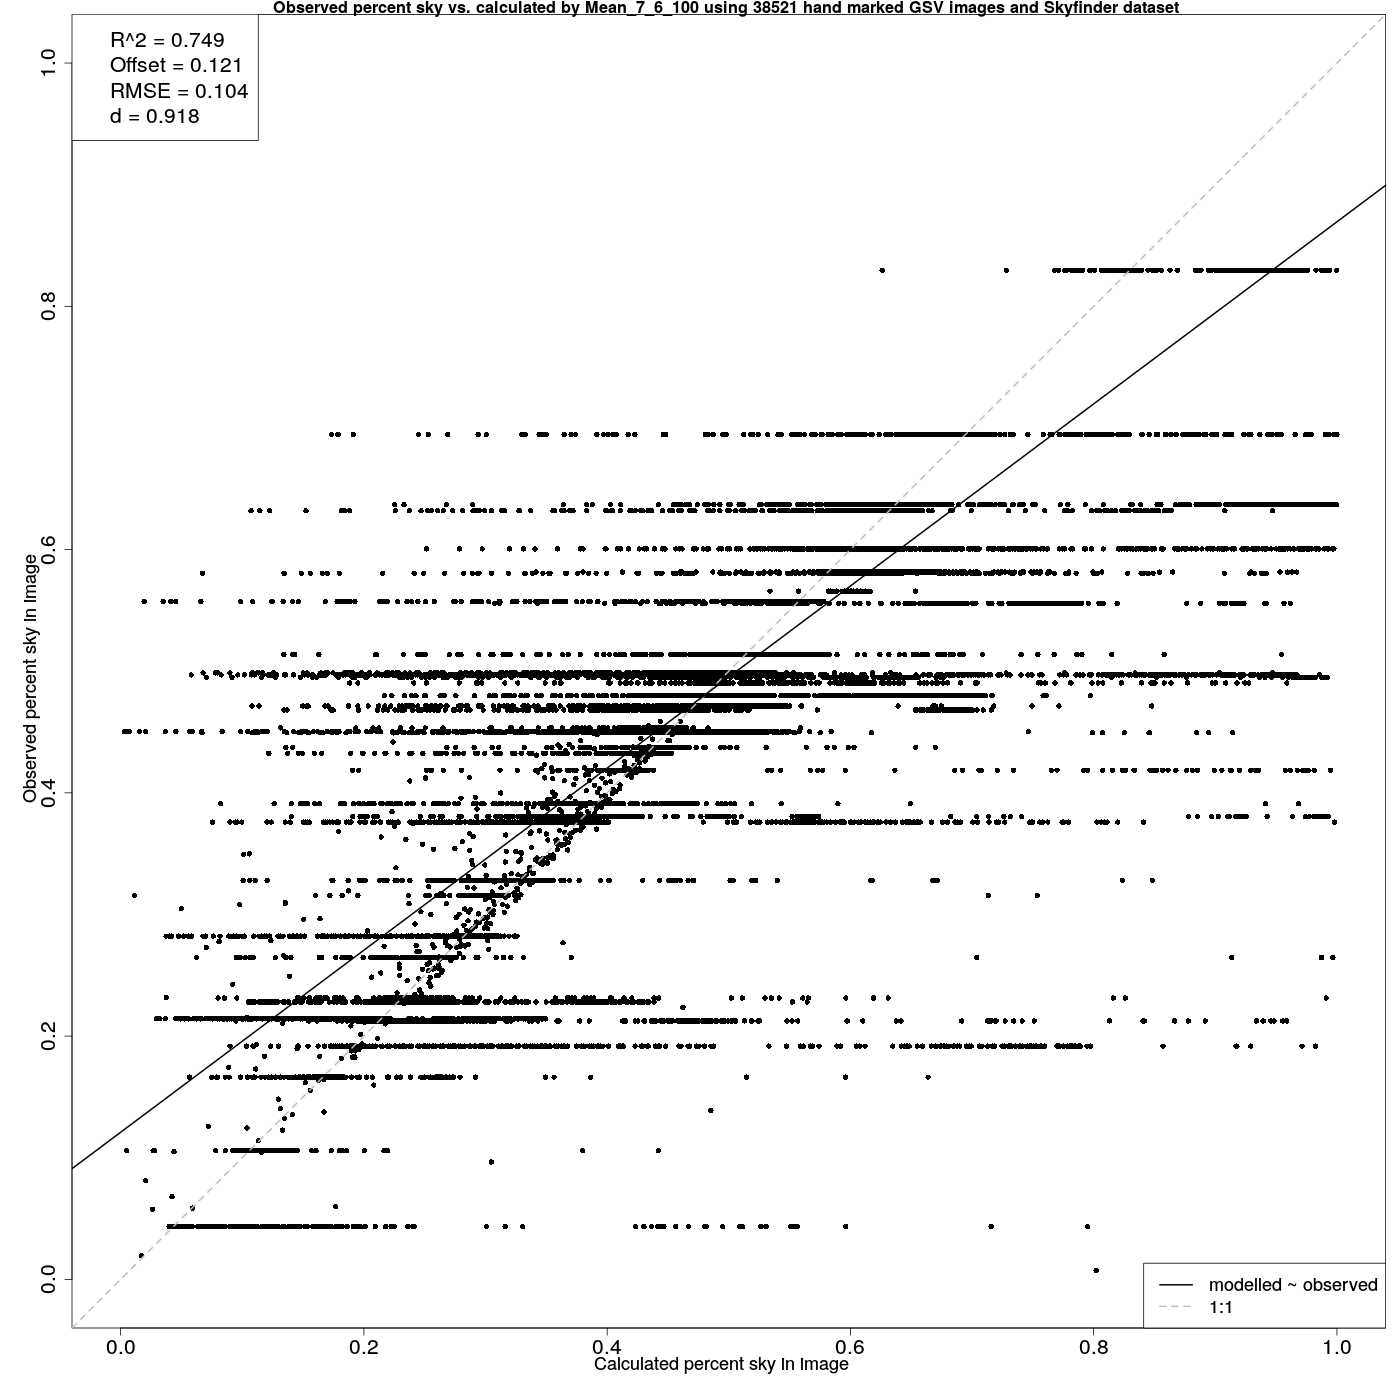
\includegraphics[scale=0.15]{Images/ErrorPlotsCombinedIndivMean_7_6_100.png} 
% R CMD BATCH /home/kerryn/git/2018-03-MasterITProject/SkyViewDetection/SkyfinderEvaluationOutput/Plots/scriptCombinedIndiv_Mean_7_6_100.R
% cp -u ../2018-03-MasterITProject/SkyViewDetection/SkyfinderEvaluationOutput/Plots/ErrorPlotsGSVandSMean_7_6_100.png Images/ErrorPlotsCombinedIndivMean_7_6_100.png
\textbf{b)}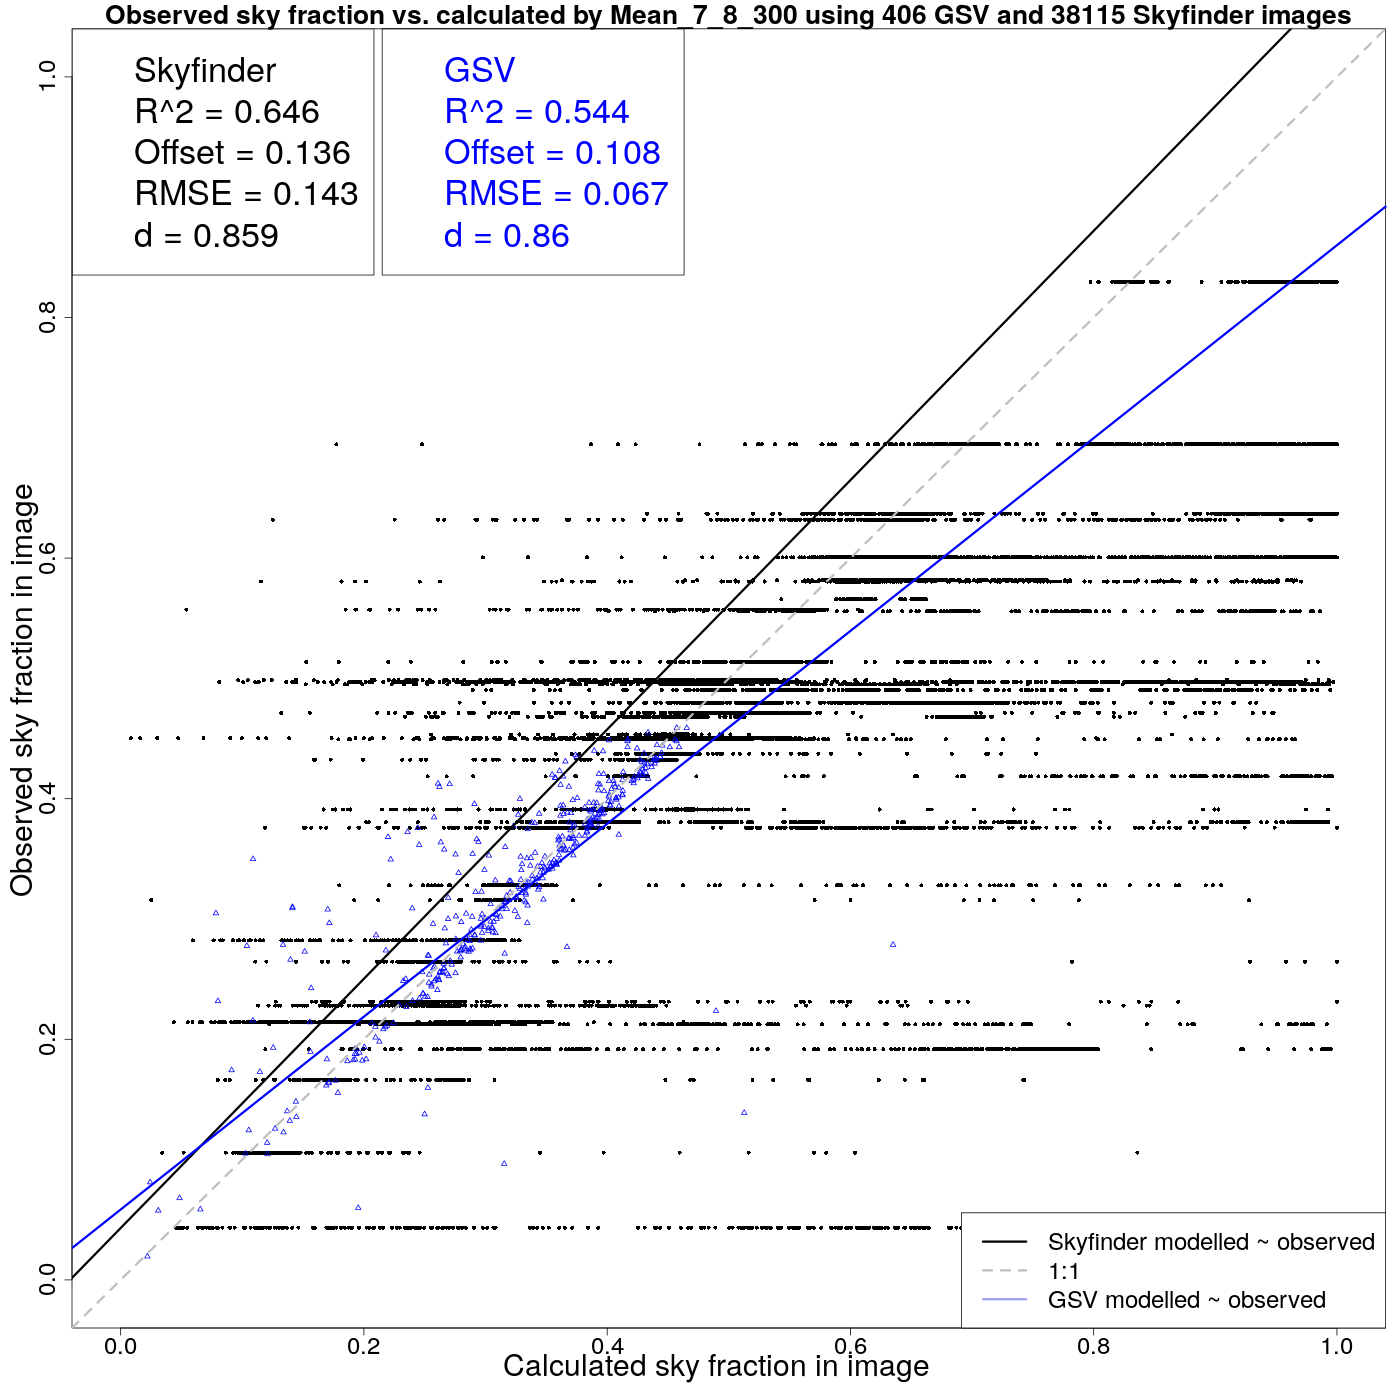
\includegraphics[scale=0.15]{Images/ErrorPlotsCombinedIndivMean_7_8_300.png}
% R CMD BATCH /home/kerryn/git/2018-03-MasterITProject/SkyViewDetection/SkyfinderEvaluationOutput/Plots/scriptCombinedIndiv_Mean_7_8_300.R
% cp -u /home/kerryn/git/2018-03-MasterITProject/SkyViewDetection/SkyfinderEvaluationOutput/Plots/ErrorPlotsGSVandSMean_7_8_300.png /home/kerryn/git/2019-01-UrbanClimateSVF/Images/ErrorPlotsCombinedIndivMean_7_8_300.png
\textbf{c)}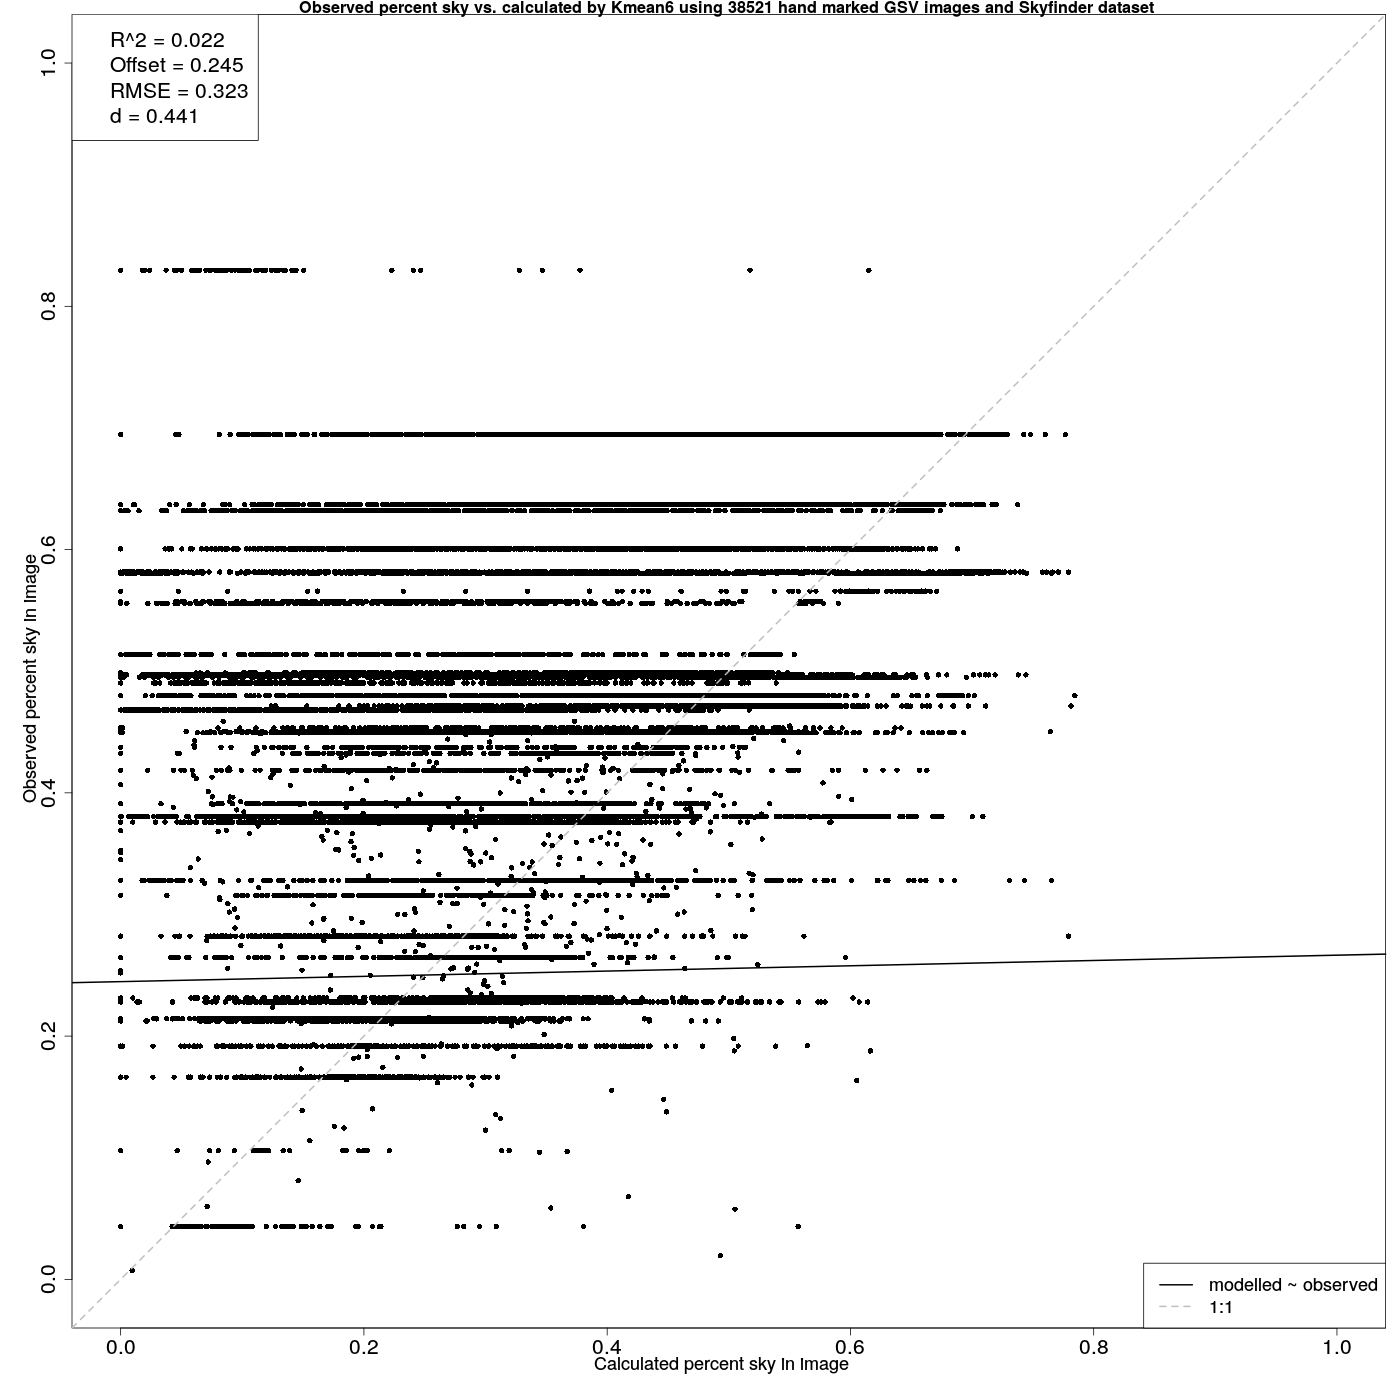
\includegraphics[scale=0.15]{Images/ErrorPlotsCombinedIndivKmean6.png}
% R CMD BATCH /home/kerryn/git/2018-03-MasterITProject/SkyViewDetection/SkyfinderEvaluationOutput/Plots/scriptCombinedIndiv_Kmean6.R
% cp -u /home/kerryn/git/2018-03-MasterITProject/SkyViewDetection/SkyfinderEvaluationOutput/Plots/ErrorPlotsGSVandSKmean6.png /home/kerryn/git/2019-01-UrbanClimateSVF/Images/ErrorPlotsCombinedIndivKmean6.png
\textbf{d)}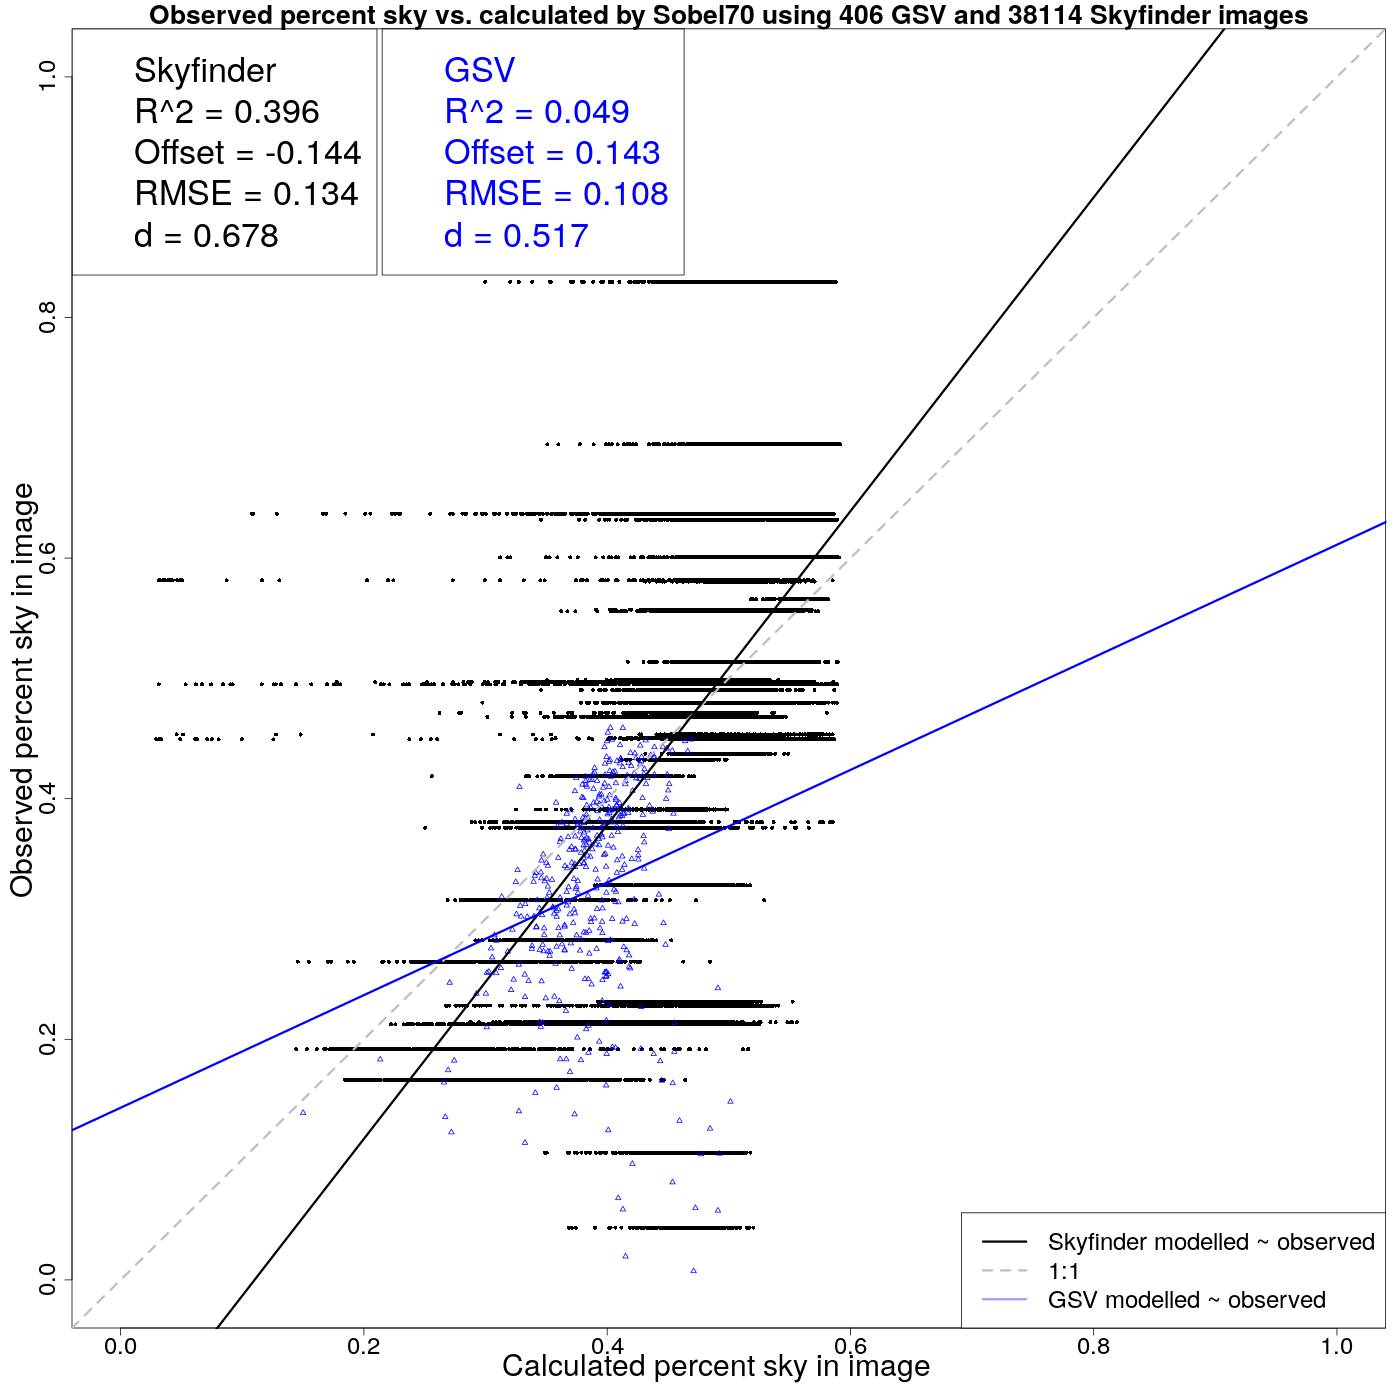
\includegraphics[scale=0.15]{Images/ErrorPlotsCombinedIndivSobel70.png}
% R CMD BATCH /home/kerryn/git/2018-03-MasterITProject/SkyViewDetection/SkyfinderEvaluationOutput/Plots/scriptCombinedIndiv_Sobel70.R
% cp -u /home/kerryn/git/2018-03-MasterITProject/SkyViewDetection/SkyfinderEvaluationOutput/Plots/ErrorPlotsGSVandSSobel70.png /home/kerryn/git/2019-01-UrbanClimateSVF/Images/ErrorPlotsCombinedIndivSobel70.png
\caption{\textbf{Observed vs. calculated sky pixels using the a) Mean\_7\_6\_100, b) Mean\_7\_8\_300, c) K-mean\_6, and d) Sobel\_70 techniques on the 38,521 image combined dataset.} }
\label{fig:errorallcombined}
\end{figure}

\subsection{Results from neural network classified techniques}\label{sec:resultsnn}
Figure \ref{fig:errorplots}a presents a theoretical best case. If the NN was 100\% accurate in picking the best technique from the thirteen possible combinations based on its training, a RMSE of 0.026 and 0.02 is possible against the 38,115 Skyfinder images and 406 GSV images respectively. 

\begin{figure}
\centering
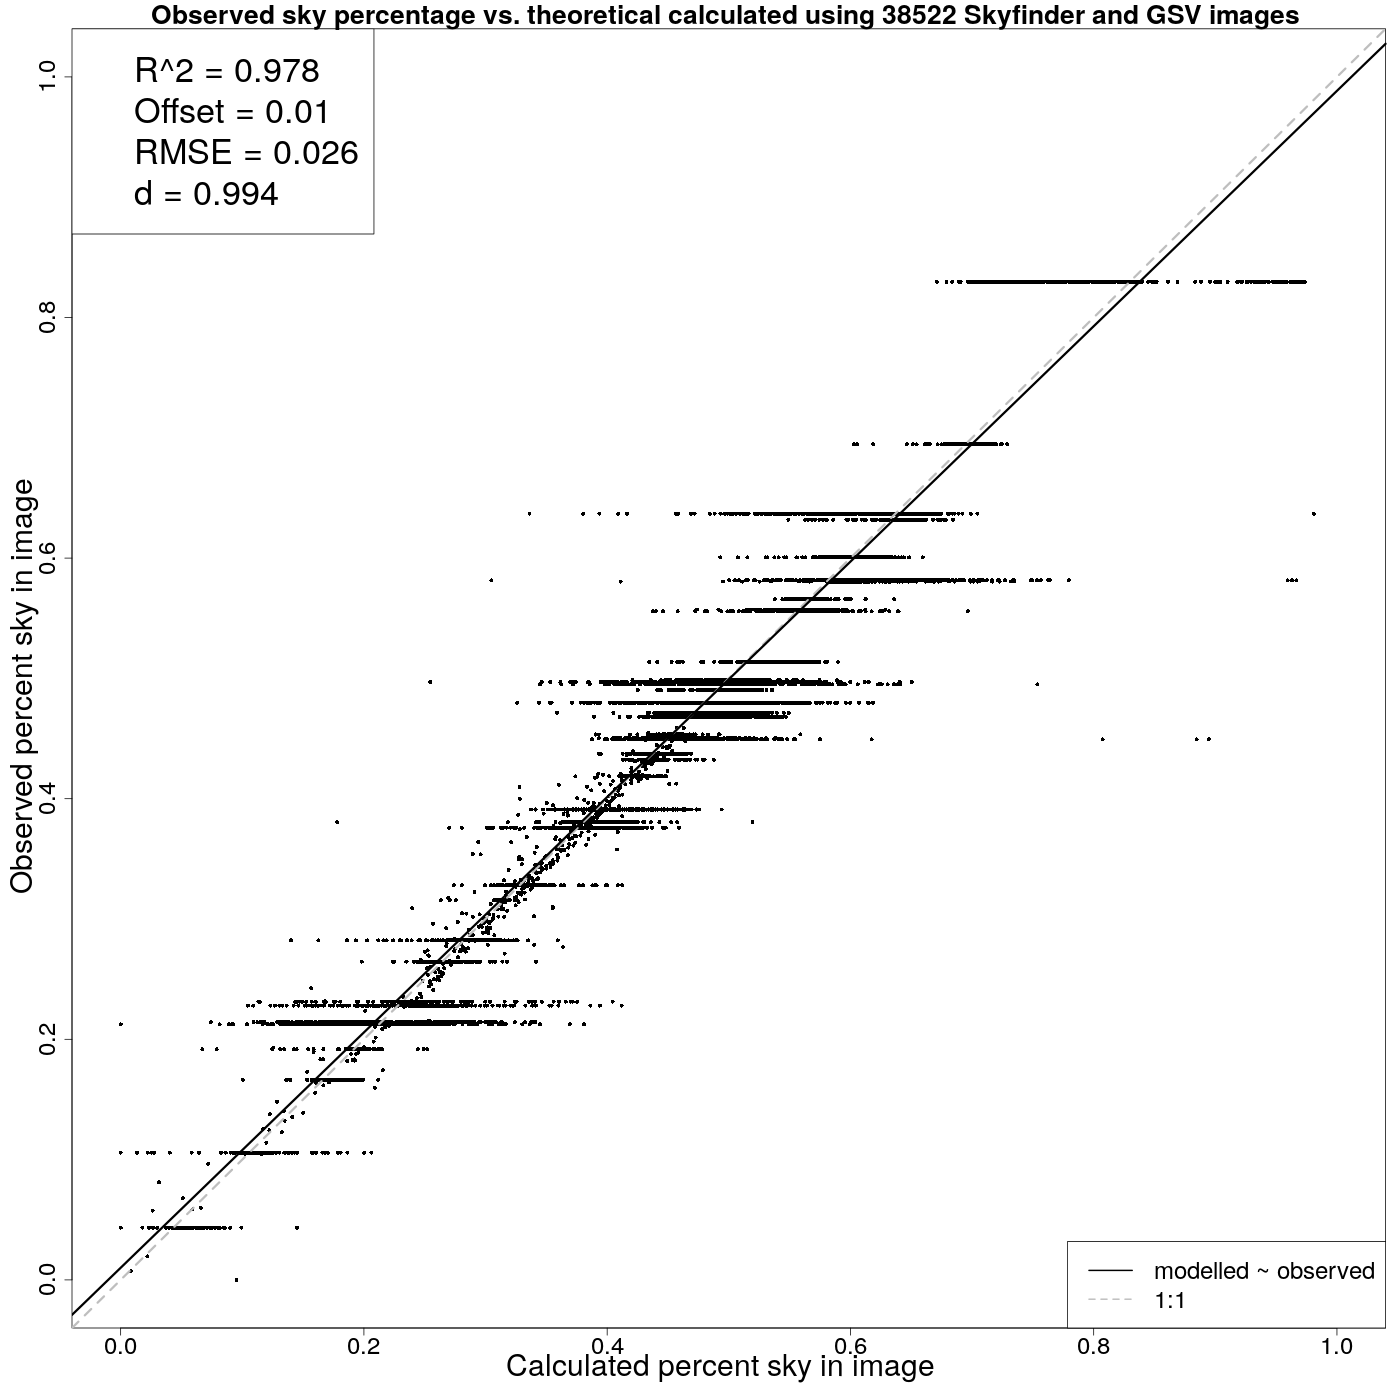
\includegraphics[scale=0.15]{Images/ErrorPlots1Combined.png}
% AnalyzeResults2ReprocessTheory.java
% R CMD BATCH /home/kerryn/git/2018-03-MasterITProject/SkyViewDetection/SkyfinderEvaluationOutput/Plots/scriptReprocess2Theory.R
% cp -u /home/kerryn/git/2018-03-MasterITProject/SkyViewDetection/SkyfinderEvaluationOutput/Plots/ErrorPlots2Reprocess2Theory.png /home/kerryn/git/2019-01-UrbanClimateSVF/Images/ErrorPlots1Combined.png 

\caption{\textbf{
Theoretical best case results if the NN is 100\% accurate for the 9636 validation images. 
%b) Results of NN picks against the 9636 validation images.
}}
\label{fig:errorplotscntk} \label{fig:errorplots}
\end{figure}

Samples of the imagery used in training for selected classifications are shown in Figure \ref{fig:classImages}. As can be seen in this figure, there are no strong visual themes in each of the classifications (i.e. all very cloudy, clear blue sky, or multi-coloured sky), however the NN is able to pick up on  more subtle features not readily visible to the eye. 

\begin{figure}
\centering
\textbf{a)}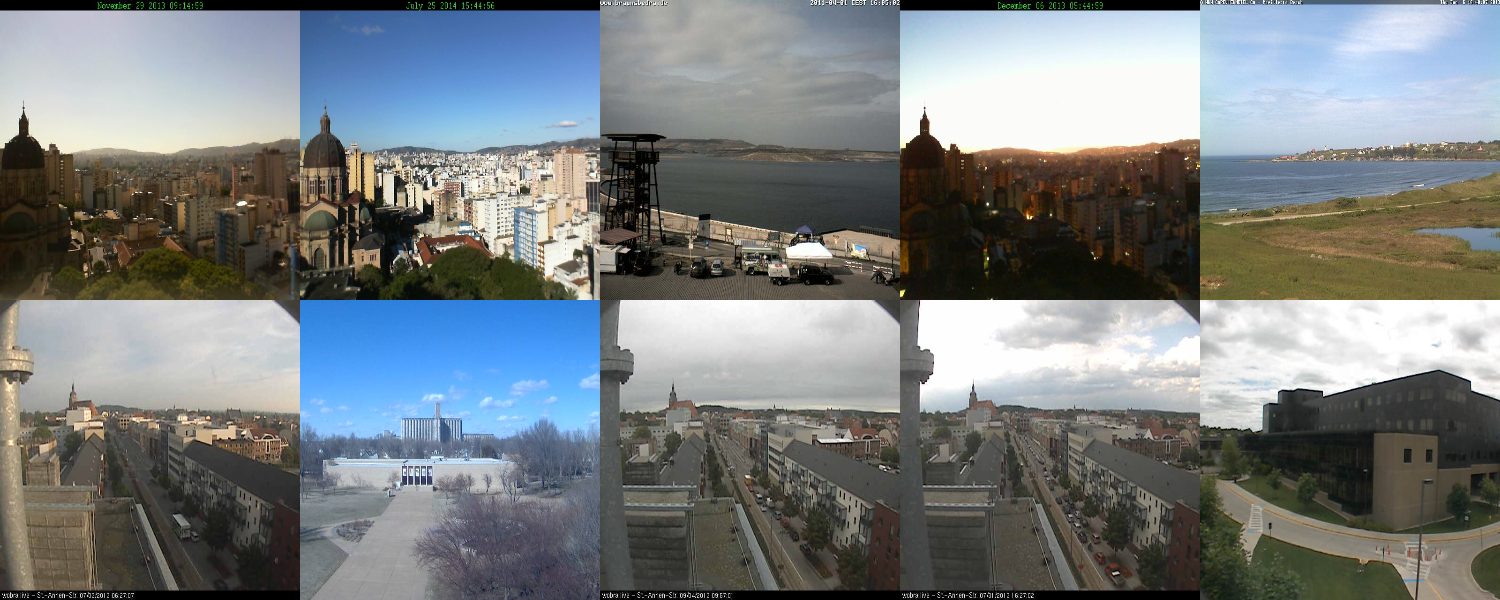
\includegraphics[trim = 0mm 0mm 0mm 0mm,clip,scale=0.14]{Images/13-0_Mean_7_8_300_tiles.png}
\textbf{b)}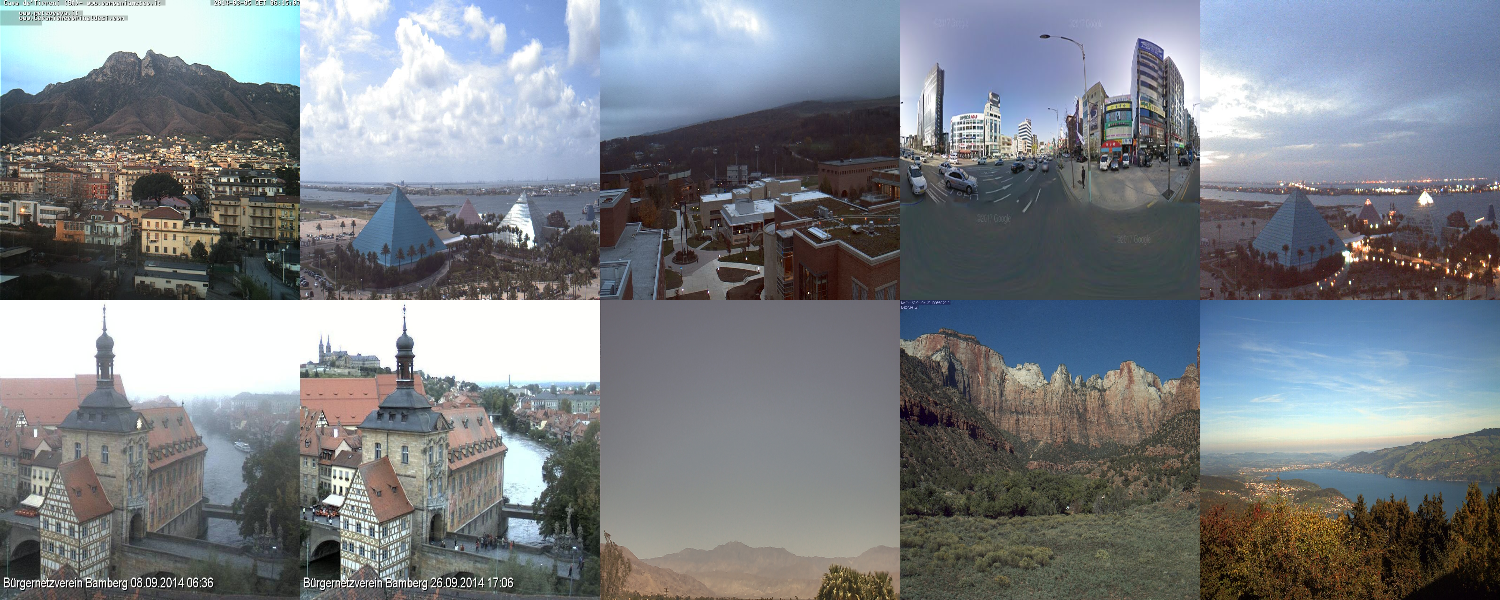
\includegraphics[trim = 0mm 0mm 0mm 0mm,clip,scale=0.14]{Images/13-3_Mean_7_6_100_tiles.png}
\textbf{c)}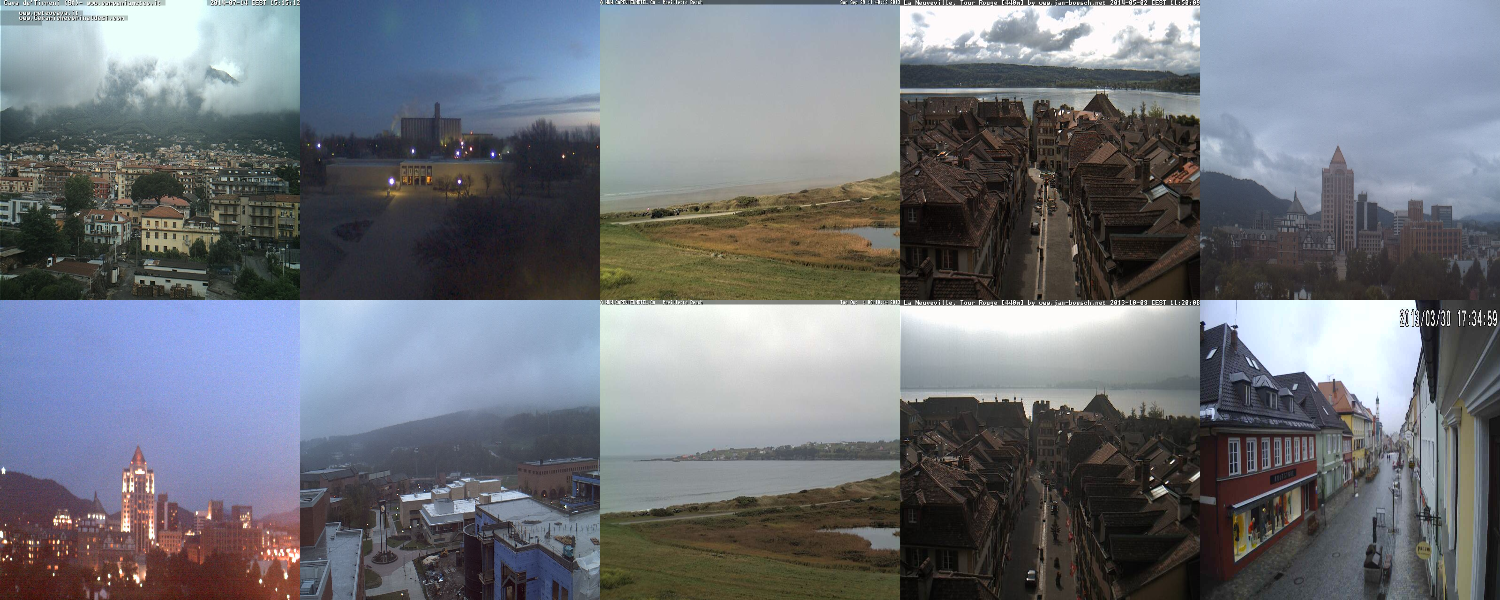
\includegraphics[trim = 0mm 0mm 0mm 0mm,clip,scale=0.14]{Images/13-5_K-mean_6_tiles.png}
\textbf{d)}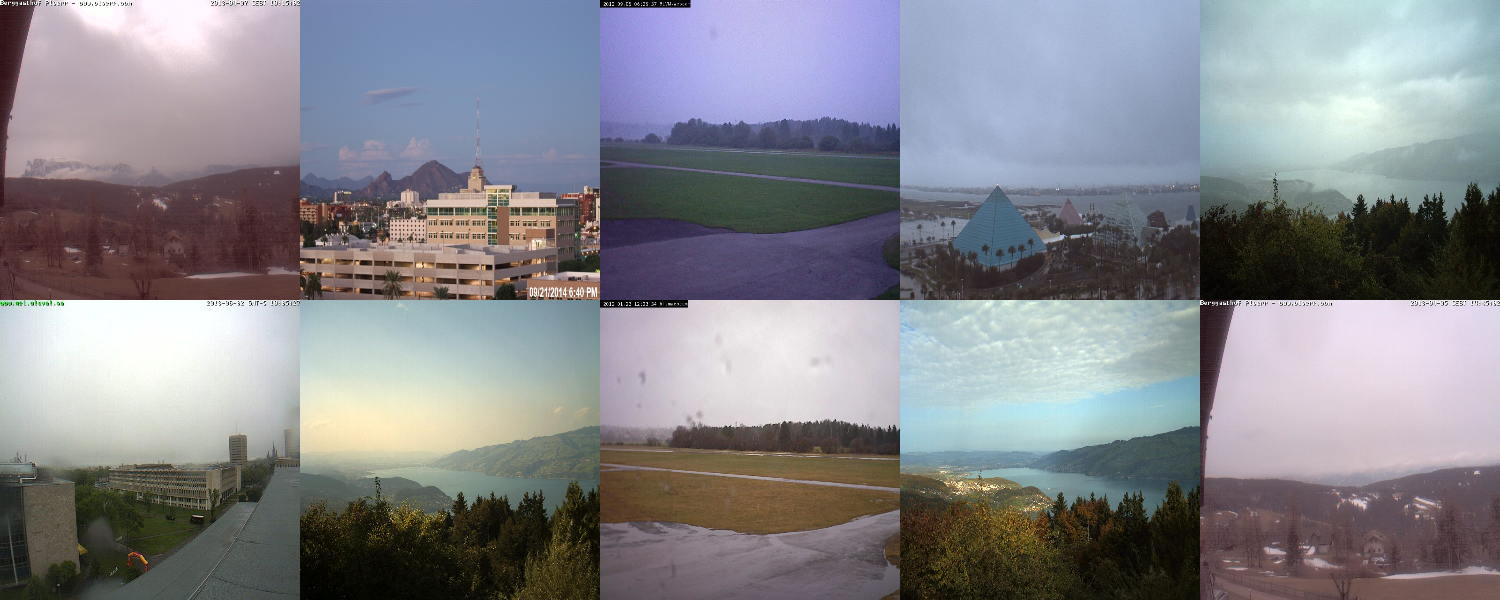
\includegraphics[trim = 0mm 0mm 0mm 0mm,clip,scale=0.14]{Images/13-9_Sobel_70_tiles.png}
\caption{\textbf{Selected imagery used for NN training for classifications 
a) Mean\_7\_8\_300, b) Mean\_7\_6\_100, c) K-mean\_6, d) Sobel\_70.}}
\label{fig:classImages}
\end{figure}

The neural network was trained for 250 epochs on a Nvidia GeForce GTX 1080 GPU, requiring about 12 hours. The neural network reached peak error rate of 46.3\% in choosing between the 13 classifications. However, as the classification results were more of a continuum, where some techniques did only slightly better than others, a strictly binary choice is not always necessary. Breaking down the accuracy with this in mind, the NN reached 52.6\% accuracy in picking the best method, 18.9\% accurate in picking the second best method, and 10.5\% in picking the third best method (for a total of the three of 82.0\%)

Figure \ref{fig:errorplotscntk}b shows the overall accuracy of the NN chosen pathway process flow against the 9636 validation images, with a RMSE of 0.063 and R$^{2}$ of 0.879. The accuracy of the NN has impacted the overall accuracy of the system (i.e. not reaching the theoretical accuracy of 0.026 or 0.02 RMSE), but the results are still very good. 





%  Finished Epoch[249 of 250]: [Validate] ce = 3.94070510 * 9529; errs = 46.259% * 9529; top5Errs = 7.923% * 9529
%first best=5227 = 0.52606682769726247987
%second best=1878 = 0.18900966183574879227
%third best=1049 = 0.10557568438003220611
%not best=1782 = 0.17934782608695652173
%total=9936
%   first accuracy 52.6%, second 18.9%, third 10.5%, total of three 82.0%





%\begin{figure}
%\centering
%%\textbf{a)}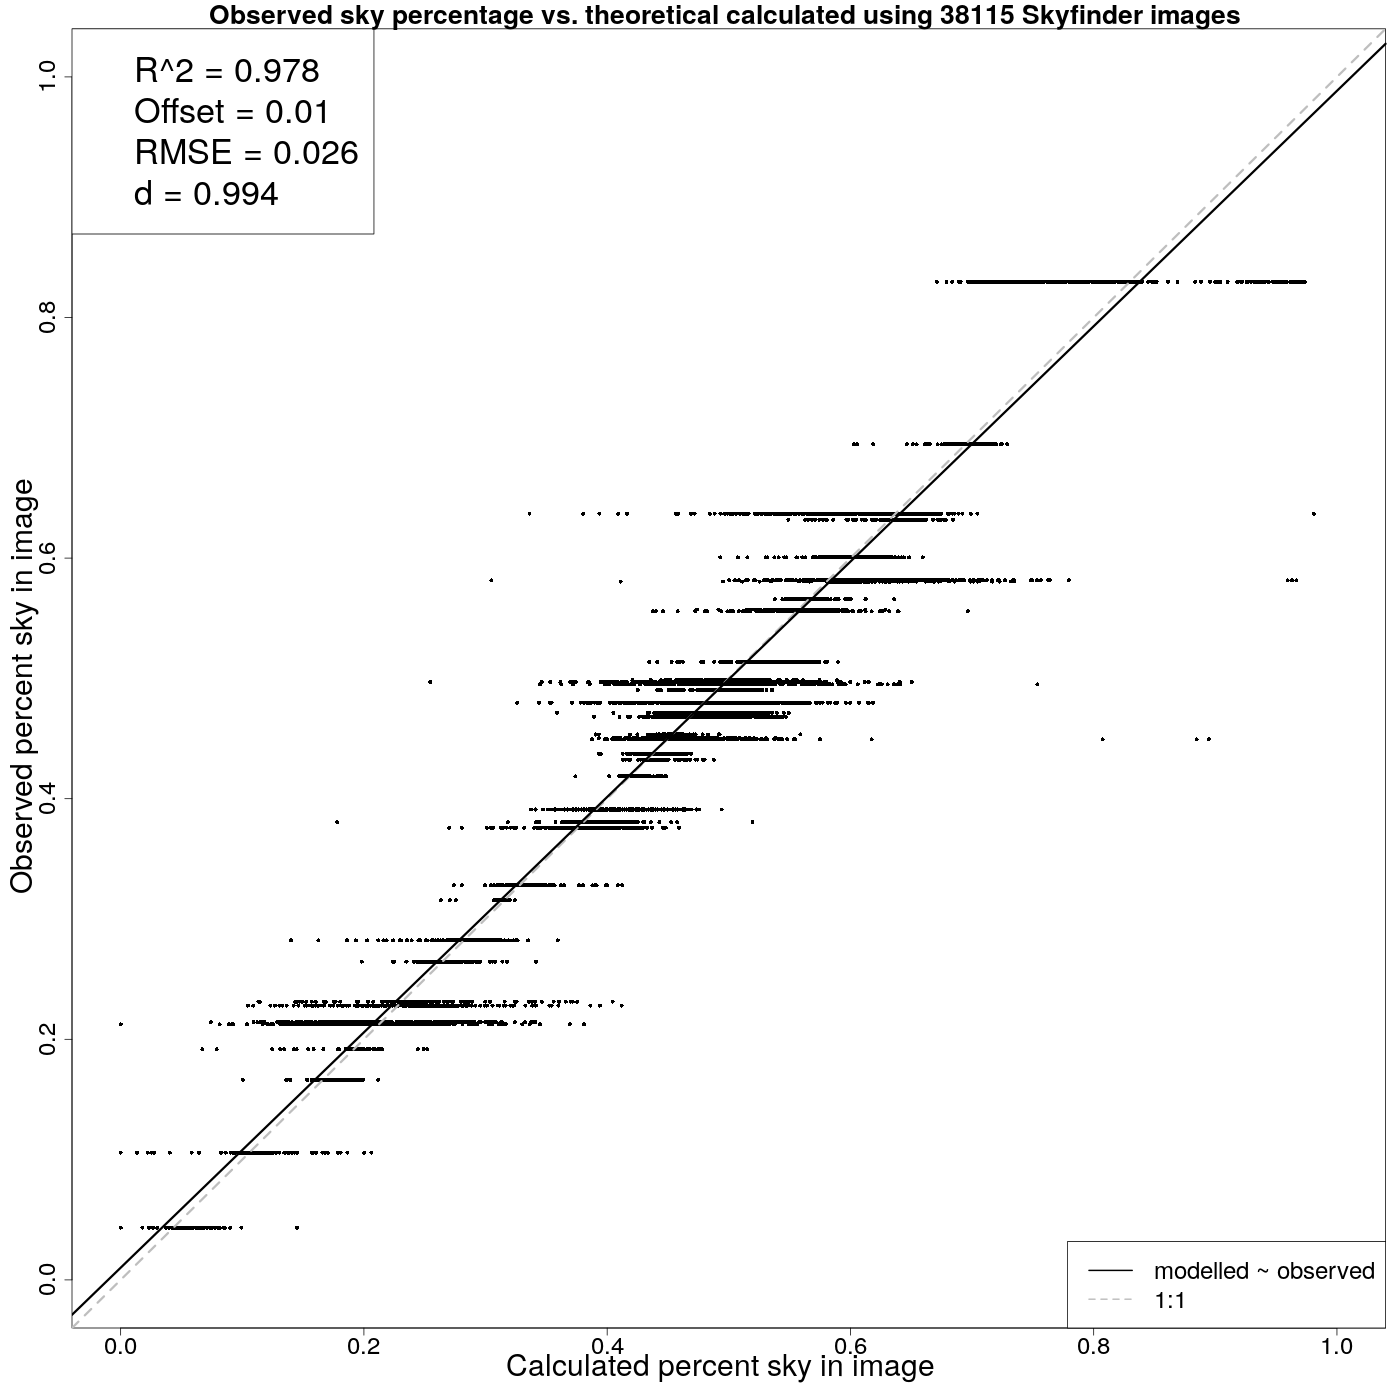
\includegraphics[scale=0.15]{Images/ErrorPlots.png}
%%\textbf{b)}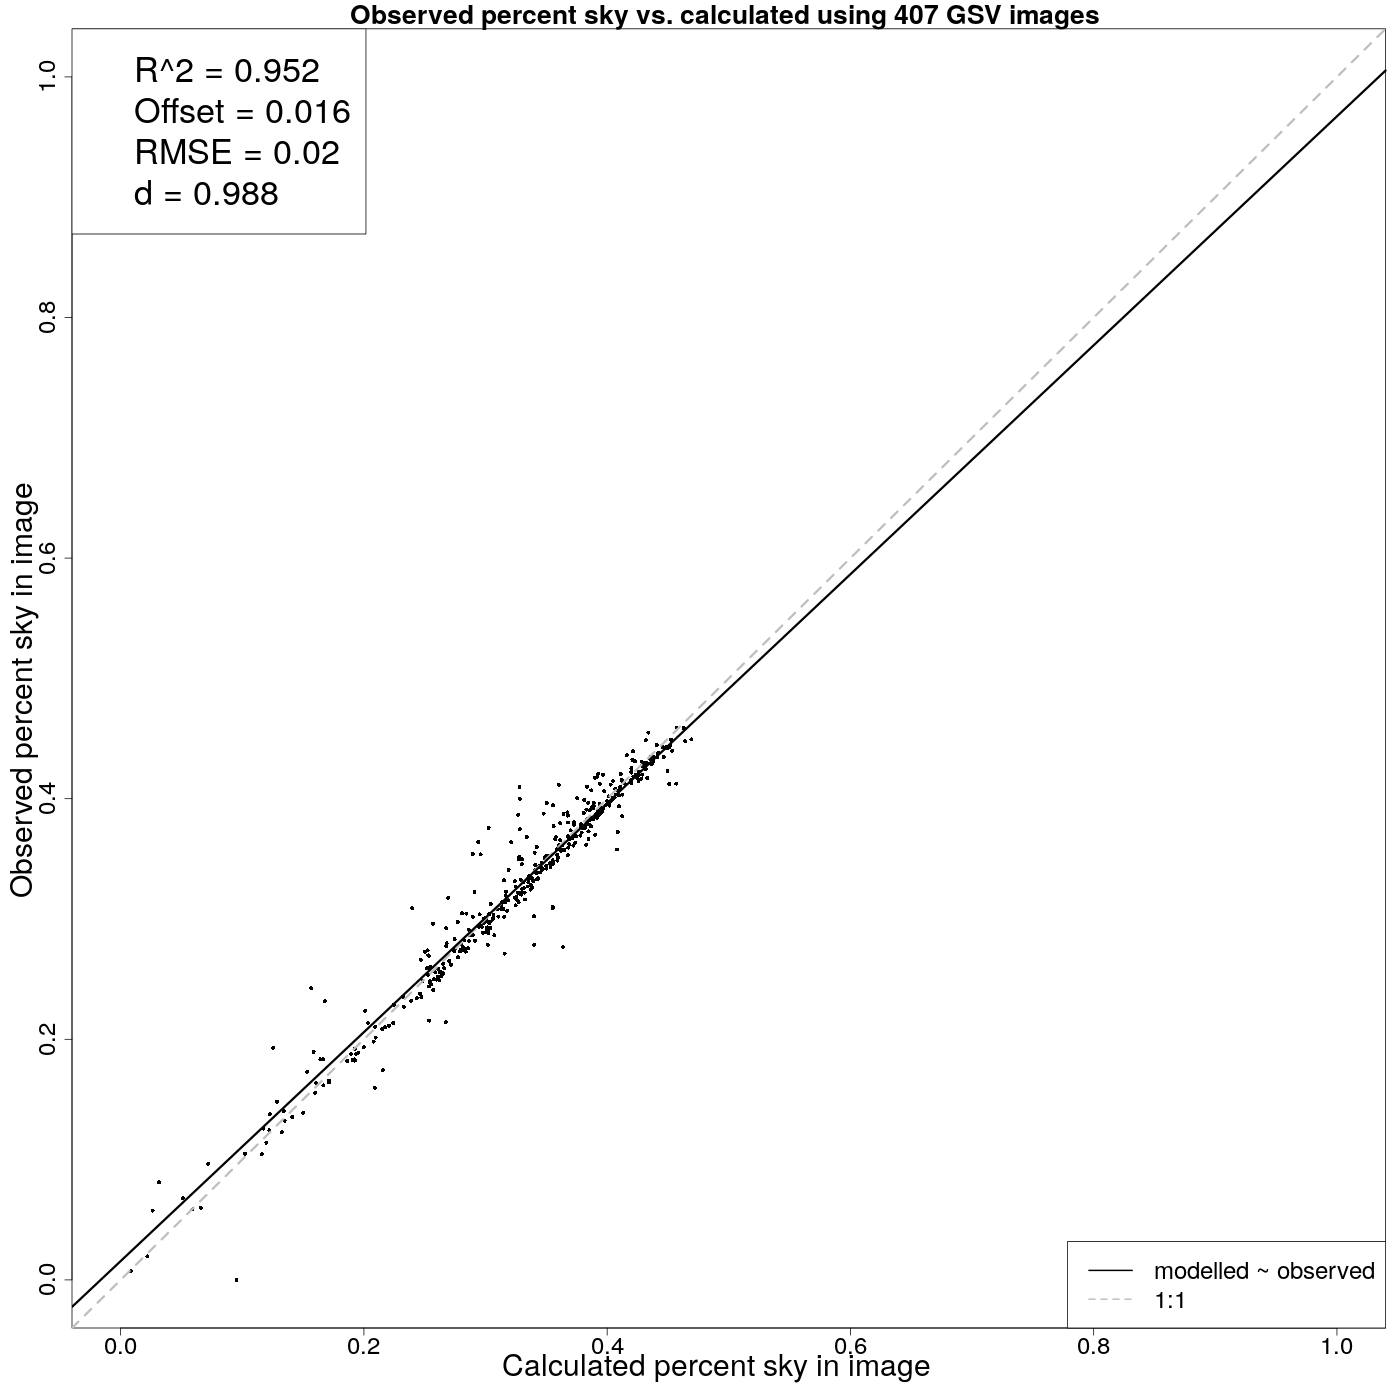
\includegraphics[scale=0.15]{Images/ErrorPlots2.png}
%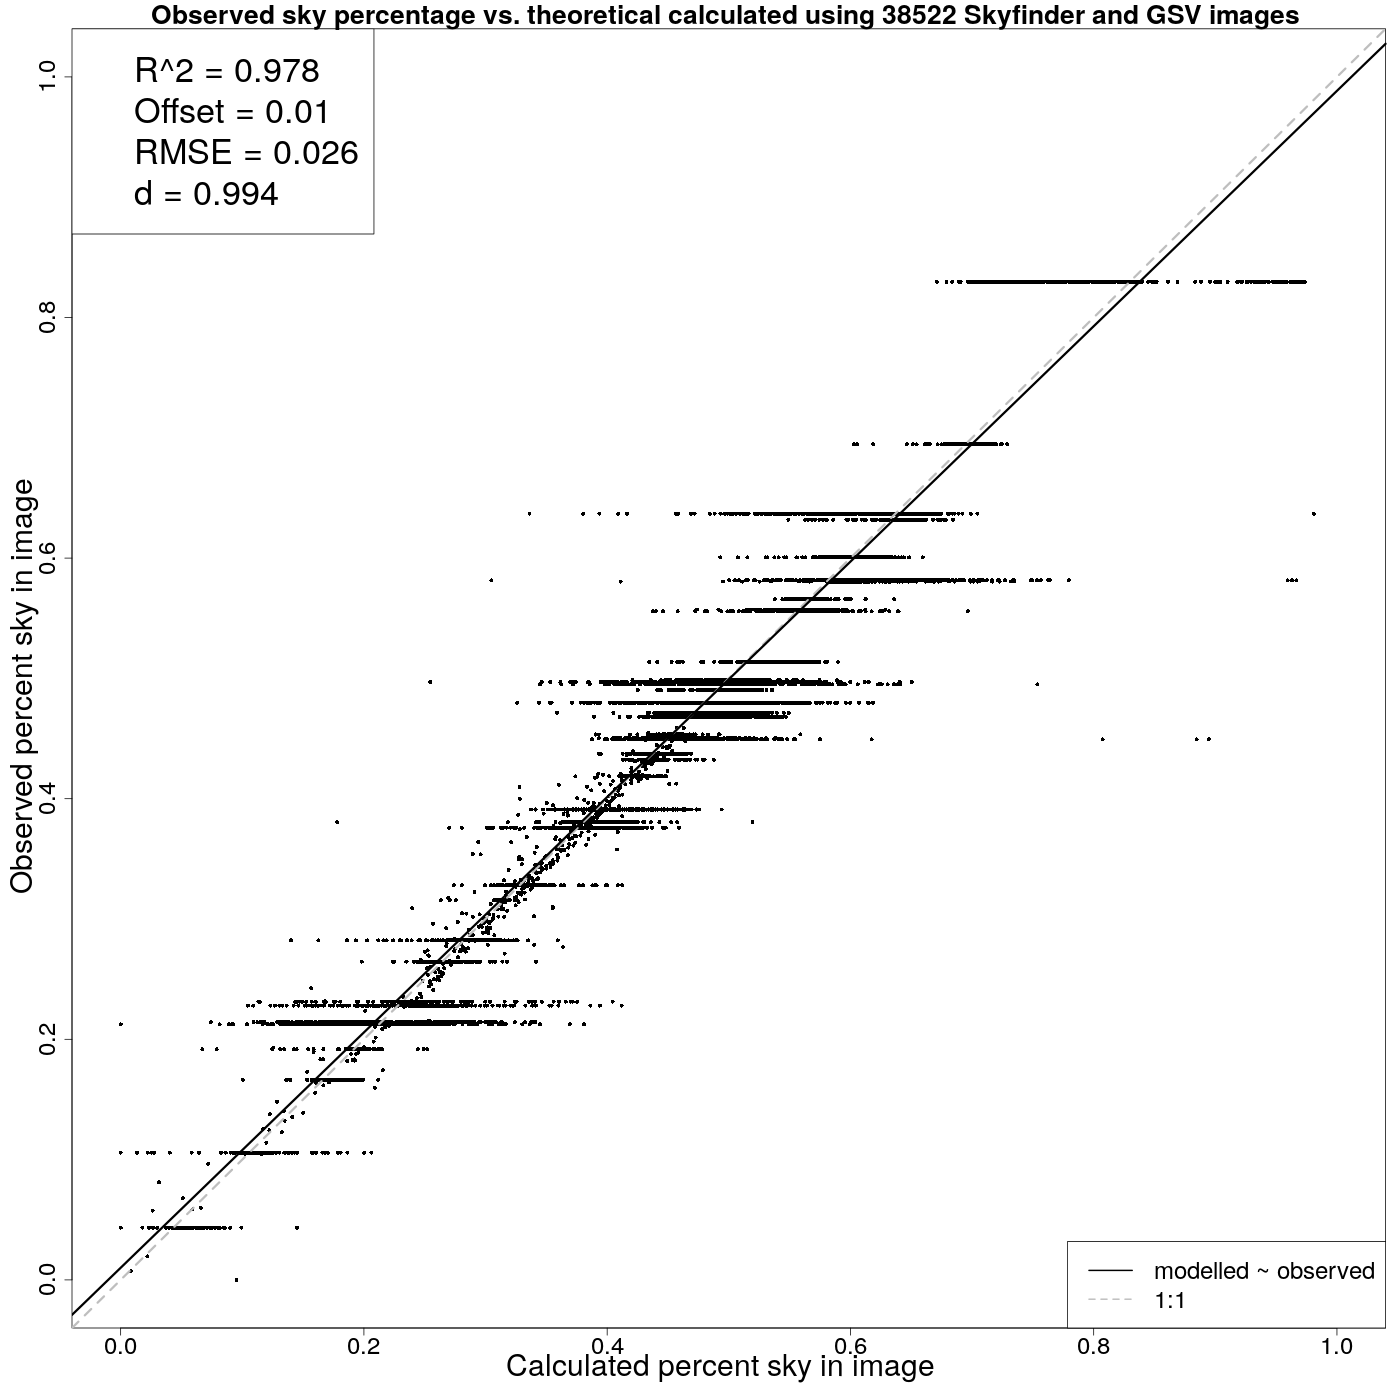
\includegraphics[scale=0.15]{Images/ErrorPlots1Combined.png}
%\caption{\textbf{Theoretical best case results if the NN is 100\% accurate for a) Skyfinder, b) GSV datasets, and c) combined datasets.}}
%\label{fig:errorplots}
%\end{figure}


%\begin{figure}
%\centering
%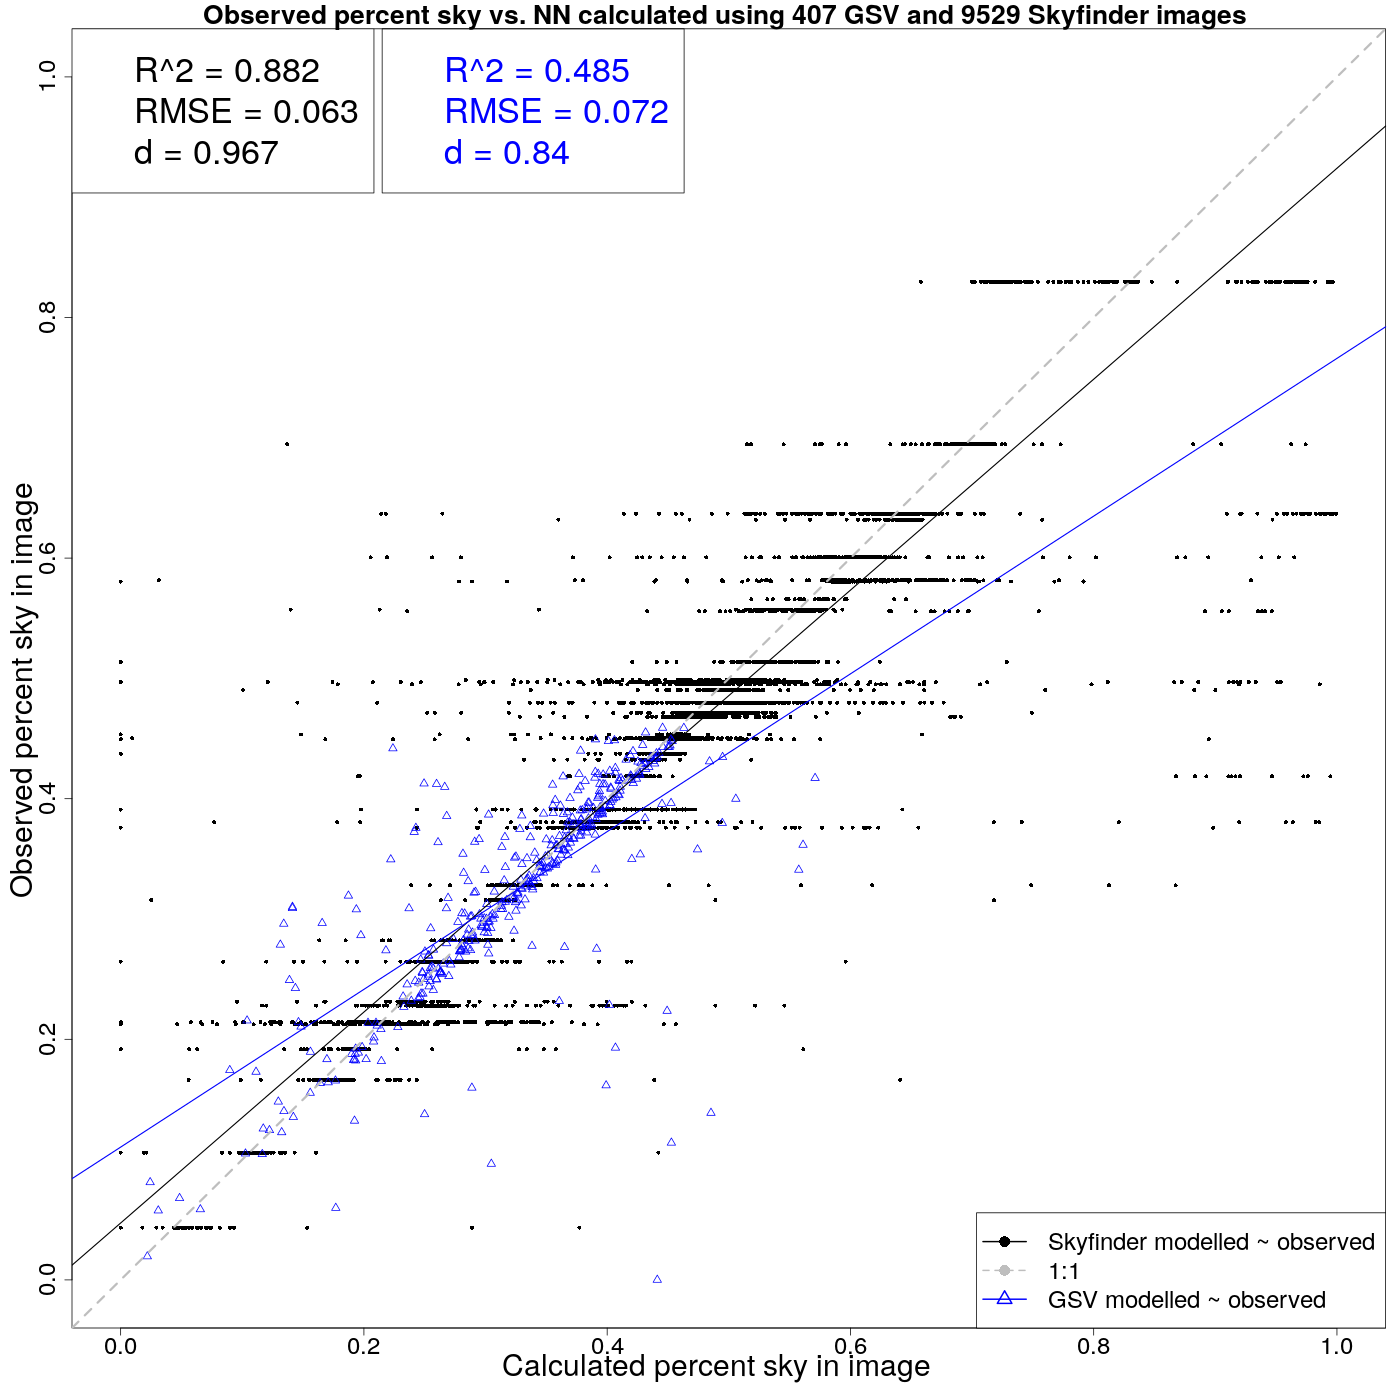
\includegraphics[scale=0.15]{Images/ErrorPlotsCNTK.png}
%\caption{\textbf{Results of NN picks against the 9636 validation images.}}
%\label{fig:errorplotscntk}
%\end{figure}

\subsection{Benchmark results}
\subsubsection{Results from the \cite{Wang2015a} Sobel operator/hybrid probability model}
These results have previously been presented in Table \ref{tab:evalall} and Figure \ref{fig:errorallcombined}. The best performing variation (Sobel\_70) for the Skyfinder data resulted in a RMSE of 0.134 and R$^{2}$ of 0.396 while the best performing variation (Sobel\_80) for the GSV data resulted in a RMSE of 0.07 and R$^{2}$ of 0.433.

\subsubsection{Results from the \cite{Middel2018} Sobel operator/flood-fill algorithm evaluation}\label{sec:resultsflood}
In the evaluation of the Sobel/flood-fill algorithm, results from the Skyfinder and GSV datasets and 9636 validation images are shown in Figure \ref{fig:errorfloodall} and Table \ref{tab:evalall}. This algorithm shows a RMSE of 0.211 and R$^{2}$ of 0.134 against with the Skyfinder images, a RMSE of 0.312 and R$^{2}$ of 0.067 against with the GSV images, and a RMSE of 0.205 and R$^{2}$ of 0.15 against the validation dataset. The results from the evaluation of GSV imagery showed a number of images miss marked as 100\% sky, inflating the error rate for this dataset. A similar problem was seen with the Skyfinder images, many of them were miss marked as 0\% sky.


\begin{figure}
\centering
\textbf{a)}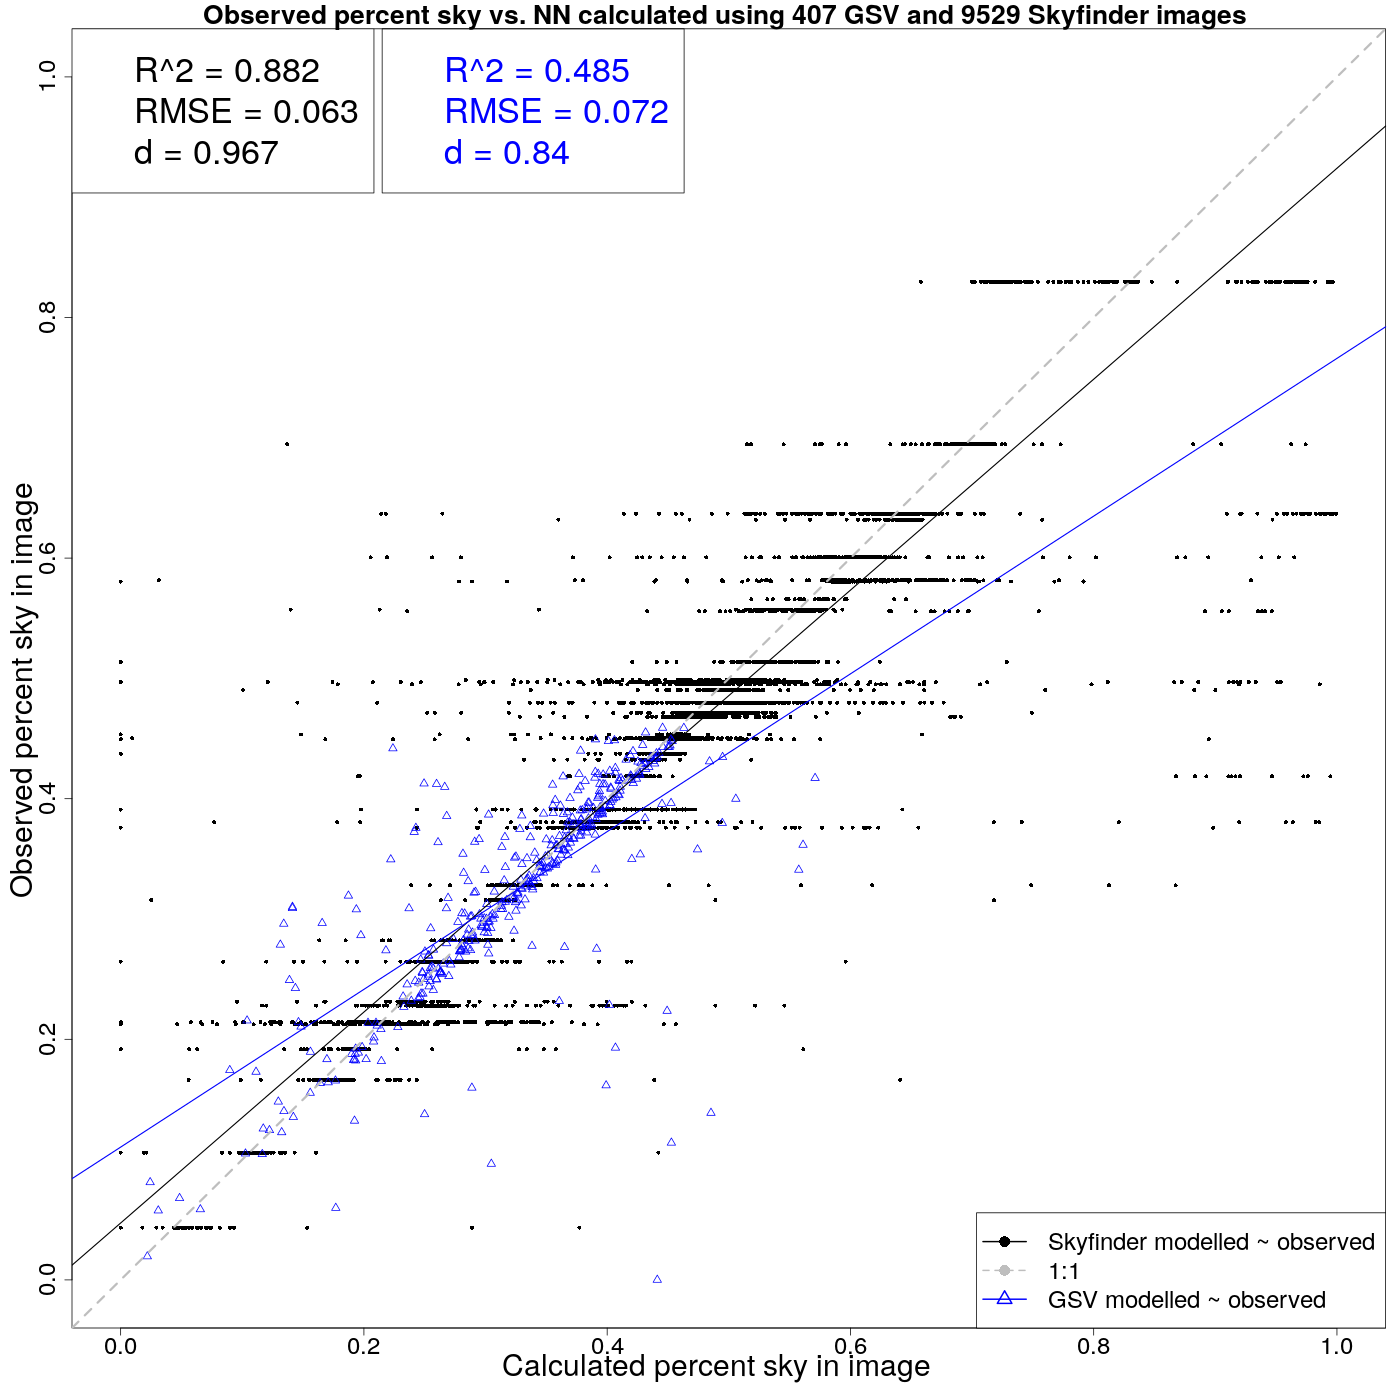
\includegraphics[scale=0.15]{Images/ErrorPlotsCNTK.png}
% AnalyzeCNTKResults.java
% R CMD BATCH /home/kerryn/git/2018-03-MasterITProject/SkyViewDetection/SkyfinderEvaluationOutput/Plots/scriptCNTK_13classesSkyfinderGSVEp249.R
% cp -u /home/kerryn/git/2018-03-MasterITProject/SkyViewDetection/SkyfinderEvaluationOutput/Plots/ErrorPlotsCNTK13classesSkyfinderGSVEp249_2.png /home/kerryn/git/2019-01-UrbanClimateSVF/Images/ErrorPlotsCNTK.png 
\textbf{b)}\includegraphics[scale=0.15]{Images/ErrorPlotsGSVandSSobel70val.png}
% AnalyzeResultsForGSVIndivTechniques2.java
% String imageSuffix= "Sobel70";
% R CMD BATCH /home/kerryn/git/2018-03-MasterITProject/SkyViewDetection/SkyfinderEvaluationOutput/Plots/scriptCombinedIndivVal_Sobel70.R
%  cp -u /home/kerryn/git/2018-03-MasterITProject/SkyViewDetection/SkyfinderEvaluationOutput/Plots/ErrorPlotsGSVandSSobel70val.png  /home/kerryn/git/2019-01-UrbanClimateSVF/Images/ErrorPlotsGSVandSSobel70val.png 
\textbf{c)}\includegraphics[scale=0.15]{Images/ErrorPlots2FloodfillValidation.png}
% FloodfillEvaluation.java
% R CMD BATCH /home/kerryn/git/2018-03-MasterITProject/SkyViewDetection/SkyfinderEvaluationOutput/Plots/scriptFloodfillValidationSplitFloodfillValidationSplit.R
% cp -u /home/kerryn/git/2018-03-MasterITProject/SkyViewDetection/SkyfinderEvaluationOutput/Plots/ErrorPlots2SplitFloodfillValidationSplit.png /home/kerryn/git/2019-01-UrbanClimateSVF/Images/ErrorPlots2FloodfillValidation.png 
\caption{\textbf{
Results against the 9636 validation images using a) our adaptive NN process, b) Benchmark 1: Sobel\_70, and c) Benchmark 2: Sobel/flood-fill combination.}}
\label{fig:errorfloodall}
\end{figure}


\section{Discussion and conclusion}\label{sec:conclusion}

In comparison to published methods, the adaptive process performs well. Our accuracy of RMSE of 0.063 compares well to the RMSE of 0.205 for the \cite{Middel2018} Sobel/flood-fill algorithm and the best performing \cite{Wang2015a} Sobel variations, Sobel\_70 and Sobel\_80, which achieved an RMSE of 0.134 and 0.07.

The results from Section \ref{sec:resultsall} show that no single technique and parameter combination performs sky pixel identification with high accuracy across the dataset used by this project. This dataset contains a wide variety of outdoor scenes with a wide range of lighting and weather conditions (as can be seen in some of the sample images in Figure \ref{fig:classImages}), challenging many of the techniques. 

It was expected that all the algorithms would perform better with GSV imagery, due to their regularity. These images were captured with the same type of equipment, using the same camera angles (horizon at 50\% image height), under clear sky or partly cloudy conditions. The results show that almost all of the variations perform better with the GSV data than the Skyfinder data. Some of the variations even approach the accuracy of our system with the GSV data, for example Sobel\_80. 

However, the Skyfinder dataset challenged all of the variations with the Mean and Sobel based methods achieving no better than 0.1 to 0.2 RMSE. However, for some individual images, even the poorest performing techniques excelled compared to all of the other techniques. Also, in some cases, some techniques perform poorly for certain images. In Figure \ref{fig:errorallcombined}d, the results for the Sobel\_70 method show wide variations in $R^{2}$ between the Skyfinder and GSV datasets while the RMSE values are roughly similar. In the case of Sobel\_70, sky fractions for images with low sky fractions (a small number of images in the dataset) are systematically overestimated but this has a dramatic impact on the GSV $R^{2}$ values. Both of these cases validates the need to have an adaptive process that can respond to the specific challenges each image presents to deliver overall better results than any single algorithm, also allowing certain techniques to be not chosen in the cases that they will perform poorly.

Further, having a range of combinations of techniques was important for the overall accuracy. Experimentation was preformed to reduce the number of classifications to possibly increase the accuracy of the NN (reducing the number of the required classifications choices). However, in removing some of the worst performing methods (many of the K-means variations), the overall accuracy degraded. While some of the variations had very low accuracy overall, in processing some images, they were the best choice and having those available overrode the lower accuracy in the NN picking the exact best choice.

While the theoretical accuracy from the 13 classes was a RMSE of 0.026, combinations of the best performing three or four classes saw reduced theoretical accuracy reduced to RMSEs of 0.039 (for Mean\_7\_6\_100, K-mean6, and Sobel\_70), 0.045 (for Mean\_3\_6\_100, K-mean6, and Sobel\_70), 0.036 (for Mean\_7\_6\_100, Mean\_7\_6\_100, K-mean6, and Sobel\_70), or 0.095 (for all Mean combinations). 

This attempt to increase the accuracy of the NN predictions highlights a limitation of this study. 53\% error in picking between 13 classes shows that there is room for improvement. NNs perform best when they are trained with a large amounts of data. It this study, there were only 28,000 images in the training dataset. With a larger training dataset, resulting in a lower NN error rate, it would be possible to come closer to the theoretical RMSE of 0.026 for the sky pixel identification.

In our linked Data in Brief article \citep{Nice2019Data}, we provide our trained NN, used to infer the best algorithm for any type of outdoor imagery, as well as all the training and validation imagery used in this study. This system can then be used out of the box. Or with our flexible framework, new algorithms and variations of existing algorithms can be added to the system to handle new imagery with greater accuracy. 

In conclusion, we present a system of sky pixel identification that shows high accuracy rates with varied and challenging outdoor imagery. This system sits, on one side, between algorithms that can be quickly set up and run, such as \cite{Middel2018}, but that are not as accurate with challenging datasets. On the other side of complexity are systems, such as \cite{Gong2018}, requiring a more complex trained deep learning algorithm. Our adaptive system uses the best elements of each in pursuit of the most accurate results possible.




\section{Code and availability and licensing}\label{sec:available}
Code and data are available from the corresponding author on request.


%TARGET is distributed under the Creative Commons Attribution-NonCommercial-ShareAlike 4.0 Generic (CC BY-NC-SA 4.0). TARGET code cannot be used for commercial purposes. It is available in two versions, Python or Java. The Python code can be downloaded from https://doi.org/10.5281/zenodo.1300023 or Java code is available at  https://zenodo.org/record/1310138. We recommend using the Java version as it runs faster than the Python code. 



%\printglossary[title={List of Symbols}]

\section*{Acknowledgements}
The support of the Commonwealth of Australia through the Cooperative Research Centre program is acknowledged. At Monash University, Kerry Nice was funded by the Cooperative Research Centre for Water Sensitive Cities, an Australian Government initiative. At the University of Melbourne, Kerry Nice was funded by the Transport, Health, and Urban Design (THUD) Hub and a Graham Treloar Fellowship for Early Career Researchers.
 
%\end{acknowledgements}

\section*{References}\label{sec:ref}
%% If you have bibdatabase file and want bibtex to generate the
%% bibitems, please use
%%
  \bibliographystyle{elsarticle-harv} 
  %\bibliography{library}
  \bibliography{bib}

%% else use the following coding to input the bibitems directly in the
%% TeX file.

%\begin{thebibliography}{00}
%
%%% \bibitem[Author(year)]{label}
%%% Text of bibliographic item
%
%\bibitem[ ()]{}
%
%\end{thebibliography}


%% The Appendices part is started with the command \appendix;
%% appendix sections are then done as normal sections
%\appendix
%\setcounter{table}{0}
%\renewcommand{\thetable}{A\arabic{table}}

%\subsection{}                               %% Appendix A1, A2, etc.


%%%%%%%%%% taking out parameterizations
%\section{Appendix}\label{sec:app}  
%\subsection{Additional data tables}\label{app:tables}  




%\authorcontribution{This work was developed by Kerry Nice and supervised by Andrew Coutts and Nigel Tapper. Model source code was received from Scott Krayenhoff and Remko Duursma (as acknowledged in Section \ref{sec:available}). Synthesis of this code and new code was developed by Kerry Nice. The article was written by Kerry Nice with editing and suggestions from Andrew Coutts and Nigel Tapper.}
%
%\begin{acknowledgements}
%The work described in this paper was developed during a PhD. project at Monash University. Funding for this was obtailed through the City of Melbourne, Monash University, and the CRC for Water Sensitive Cities.  
%\end{acknowledgements}

%\begin{acknowledgements}
%The support of the Commonwealth of Australia through the Cooperative Research Centre program is acknowledged.
%\end{acknowledgements}






\end{document}

\endinput
%%
%% End of file `elsarticle-template-harv.tex'.
